%% LyX 2.3.7 created this file.  For more info, see http://www.lyx.org/.
%% Do not edit unless you really know what you are doing.
\documentclass[journal,article,submit,pdftex,moreauthors]{Definitions/mdpi}
\usepackage[utf8]{inputenc}
\usepackage{float}
\usepackage{url}
\usepackage{amsmath}
\usepackage{graphicx}

\makeatletter

%%%%%%%%%%%%%%%%%%%%%%%%%%%%%% LyX specific LaTeX commands.

\Title{Adapt the parameters of RBF networks using Grammatical Evolution}

\TitleCitation{Adapt the parameters of RBF networks using Grammatical Evolution}

\Author{Ioannis G. Tsoulos$^{1,\dagger,\ddagger,*}$, Alexandros Tzallas$^{2}$,
Evangelos Karvounis$^{3}$}

\AuthorNames{Ioannis G. Tsoulos, Alexandros Tzallas, Evangelos Karvounis}

\AuthorCitation{Tsoulos, I.G.; Tzallas A; Karvounis E}


\address{$^{1}$\quad{}Department of Informatics and Telecommunications,
University of Ioannina, Greece; itsoulos@uoi.gr\\
$^{2}$\quad{}Department of Informatics and Telecommunications, University
of Ioannina, Greece; tzallas@uoi.gr\\
$^{3}\quad$Department of Informatics and Telecommunications, University
of Ioannina, Greece; ekarvounis@uoi.gr}


\corres{Correspondence: itsoulos@uoi.gr;}


\firstnote{Current address: Department of Informatics and Telecommunications,
University of Ioannina, Greece.}


\secondnote{These authors contributed equally to this work.}


\abstract{Radial basis function networks are widely used in a multitude of
applications in various scientific areas in both classification and
data fitting problems. These networks deal with the above problems
by adjusting their parameters with various optimization techniques.
However, an important issue to address is finding a satisfactory interval
of values for the network parameters before adjusting these parameters.
This paper proposes a two-stage technique, where in the first stage,
using Grammatical Evolution, rules are generated to create the optimal
value interval of the network parameters. In the second stage of the
technique, the parameters of the network are fine-tuned with some
robust global optimization method, such as a genetic algorithm. The
proposed technique was tested on a number of problems from the recent
literature and found to reduce the classification or data fitting
error by over 40\% on most datasets. Furthermore, the method appears
highly stable as increasing the number of network parameters does
not significantly affect its performance.}


\keyword{Neural networks; Genetic algorithms; Genetic programming; Grammatical
evolution}

\DeclareTextSymbolDefault{\textquotedbl}{T1}
%% Because html converters don't know tabularnewline
\providecommand{\tabularnewline}{\\}
\floatstyle{ruled}
\newfloat{algorithm}{tbp}{loa}
\providecommand{\algorithmname}{Algorithm}
\floatname{algorithm}{\protect\algorithmname}

%%%%%%%%%%%%%%%%%%%%%%%%%%%%%% Textclass specific LaTeX commands.
\newenvironment{lyxcode}
	{\par\begin{list}{}{
		\setlength{\rightmargin}{\leftmargin}
		\setlength{\listparindent}{0pt}% needed for AMS classes
		\raggedright
		\setlength{\itemsep}{0pt}
		\setlength{\parsep}{0pt}
		\normalfont\ttfamily}%
	 \item[]}
	{\end{list}}

%%%%%%%%%%%%%%%%%%%%%%%%%%%%%% User specified LaTeX commands.
%  LaTeX support: latex@mdpi.com 
%  For support, please attach all files needed for compiling as well as the log file, and specify your operating system, LaTeX version, and LaTeX editor.

%=================================================================


% For posting an early version of this manuscript as a preprint, you may use "preprints" as the journal and change "submit" to "accept". The document class line would be, e.g., \documentclass[preprints,article,accept,moreauthors,pdftex]{mdpi}. This is especially recommended for submission to arXiv, where line numbers should be removed before posting. For preprints.org, the editorial staff will make this change immediately prior to posting.

%--------------------
% Class Options:
%--------------------
%----------
% journal
%----------
% Choose between the following MDPI journals:
% acoustics, actuators, addictions, admsci, adolescents, aerospace, agriculture, agriengineering, agronomy, ai, algorithms, allergies, alloys, analytica, animals, antibiotics, antibodies, antioxidants, applbiosci, appliedchem, appliedmath, applmech, applmicrobiol, applnano, applsci, aquacj, architecture, arts, asc, asi, astronomy, atmosphere, atoms, audiolres, automation, axioms, bacteria, batteries, bdcc, behavsci, beverages, biochem, bioengineering, biologics, biology, biomass, biomechanics, biomed, biomedicines, biomedinformatics, biomimetics, biomolecules, biophysica, biosensors, biotech, birds, bloods, blsf, brainsci, breath, buildings, businesses, cancers, carbon, cardiogenetics, catalysts, cells, ceramics, challenges, chemengineering, chemistry, chemosensors, chemproc, children, chips, cimb, civileng, cleantechnol, climate, clinpract, clockssleep, cmd, coasts, coatings, colloids, colorants, commodities, compounds, computation, computers, condensedmatter, conservation, constrmater, cosmetics, covid, crops, cryptography, crystals, csmf, ctn, curroncol, currophthalmol, cyber, dairy, data, dentistry, dermato, dermatopathology, designs, diabetology, diagnostics, dietetics, digital, disabilities, diseases, diversity, dna, drones, dynamics, earth, ebj, ecologies, econometrics, economies, education, ejihpe, electricity, electrochem, electronicmat, electronics, encyclopedia, endocrines, energies, eng, engproc, ent, entomology, entropy, environments, environsciproc, epidemiologia, epigenomes, est, fermentation, fibers, fintech, fire, fishes, fluids, foods, forecasting, forensicsci, forests, foundations, fractalfract, fuels, futureinternet, futureparasites, futurepharmacol, futurephys, futuretransp, galaxies, games, gases, gastroent, gastrointestdisord, gels, genealogy, genes, geographies, geohazards, geomatics, geosciences, geotechnics, geriatrics, hazardousmatters, healthcare, hearts, hemato, heritage, highthroughput, histories, horticulturae, humanities, humans, hydrobiology, hydrogen, hydrology, hygiene, idr, ijerph, ijfs, ijgi, ijms, ijns, ijtm, ijtpp, immuno, informatics, information, infrastructures, inorganics, insects, instruments, inventions, iot, j, jal, jcdd, jcm, jcp, jcs, jdb, jeta, jfb, jfmk, jimaging, jintelligence, jlpea, jmmp, jmp, jmse, jne, jnt, jof, joitmc, jor, journalmedia, jox, jpm, jrfm, jsan, jtaer, jzbg, kidney, kidneydial, knowledge, land, languages, laws, life, liquids, literature, livers, logics, logistics, lubricants, lymphatics, machines, macromol, magnetism, magnetochemistry, make, marinedrugs, materials, materproc, mathematics, mca, measurements, medicina, medicines, medsci, membranes, merits, metabolites, metals, meteorology, methane, metrology, micro, microarrays, microbiolres, micromachines, microorganisms, microplastics, minerals, mining, modelling, molbank, molecules, mps, msf, mti, muscles, nanoenergyadv, nanomanufacturing, nanomaterials, ncrna, network, neuroglia, neurolint, neurosci, nitrogen, notspecified, nri, nursrep, nutraceuticals, nutrients, obesities, oceans, ohbm, onco, oncopathology, optics, oral, organics, organoids, osteology, oxygen, parasites, parasitologia, particles, pathogens, pathophysiology, pediatrrep, pharmaceuticals, pharmaceutics, pharmacoepidemiology, pharmacy, philosophies, photochem, photonics, phycology, physchem, physics, physiologia, plants, plasma, pollutants, polymers, polysaccharides, poultry, powders, preprints, proceedings, processes, prosthesis, proteomes, psf, psych, psychiatryint, psychoactives, publications, quantumrep, quaternary, qubs, radiation, reactions, recycling, regeneration, religions, remotesensing, reports, reprodmed, resources, rheumato, risks, robotics, ruminants, safety, sci, scipharm, seeds, sensors, separations, sexes, signals, sinusitis, skins, smartcities, sna, societies, socsci, software, soilsystems, solar, solids, sports, standards, stats, stresses, surfaces, surgeries, suschem, sustainability, symmetry, synbio, systems, taxonomy, technologies, telecom, test, textiles, thalassrep, thermo, tomography, tourismhosp, toxics, toxins, transplantology, transportation, traumacare, traumas, tropicalmed, universe, urbansci, uro, vaccines, vehicles, venereology, vetsci, vibration, viruses, vision, waste, water, wem, wevj, wind, women, world, youth, zoonoticdis 

%---------
% article
%---------
% The default type of manuscript is "article", but can be replaced by: 
% abstract, addendum, article, book, bookreview, briefreport, casereport, comment, commentary, communication, conferenceproceedings, correction, conferencereport, entry, expressionofconcern, extendedabstract, datadescriptor, editorial, essay, erratum, hypothesis, interestingimage, obituary, opinion, projectreport, reply, retraction, review, perspective, protocol, shortnote, studyprotocol, systematicreview, supfile, technicalnote, viewpoint, guidelines, registeredreport, tutorial
% supfile = supplementary materials

%----------
% submit
%----------
% The class option "submit" will be changed to "accept" by the Editorial Office when the paper is accepted. This will only make changes to the frontpage (e.g., the logo of the journal will get visible), the headings, and the copyright information. Also, line numbering will be removed. Journal info and pagination for accepted papers will also be assigned by the Editorial Office.

%------------------
% moreauthors
%------------------
% If there is only one author the class option oneauthor should be used. Otherwise use the class option moreauthors.

%---------
% pdftex
%---------
% The option pdftex is for use with pdfLaTeX. If eps figures are used, remove the option pdftex and use LaTeX and dvi2pdf.

%=================================================================
% MDPI internal commands - do not modify
\firstpage{1} 
 
\setcounter{page}{\@firstpage} 

\pubvolume{1}
\issuenum{1}
\articlenumber{0}
\pubyear{2023}
\copyrightyear{2023}
%\externaleditor{Academic Editor: Firstname Lastname} % For journal Automation, please change Academic Editor to "Communicated by"
\datereceived{}
\daterevised{ } % Comment out if no revised date
\dateaccepted{}
\datepublished{}
%\datecorrected{} % Corrected papers include a "Corrected: XXX" date in the original paper.
%\dateretracted{} % Corrected papers include a "Retracted: XXX" date in the original paper.
\hreflink{https://doi.org/} % If needed use \linebreak
%\doinum{}
%------------------------------------------------------------------
% The following line should be uncommented if the LaTeX file is uploaded to arXiv.org
%\pdfoutput=1

%=================================================================
% Add packages and commands here. The following packages are loaded in our class file: fontenc, inputenc, calc, indentfirst, fancyhdr, graphicx, epstopdf, lastpage, ifthen, lineno, float, amsmath, setspace, enumitem, mathpazo, booktabs, titlesec, etoolbox, tabto, xcolor, soul, multirow, microtype, tikz, totcount, changepage, attrib, upgreek, cleveref, amsthm, hyphenat, natbib, hyperref, footmisc, url, geometry, newfloat, caption

%=================================================================
%% Please use the following mathematics environments: Theorem, Lemma, Corollary, Proposition, Characterization, Property, Problem, Example, ExamplesandDefinitions, Hypothesis, Remark, Definition, Notation, Assumption
%% For proofs, please use the proof environment (the amsthm package is loaded by the MDPI class).

%=================================================================
% The fields PACS, MSC, and JEL may be left empty or commented out if not applicable
%\PACS{J0101}
%\MSC{}
%\JEL{}

%%%%%%%%%%%%%%%%%%%%%%%%%%%%%%%%%%%%%%%%%%
% Only for the journal Diversity
%\LSID{\url{http://}}

%%%%%%%%%%%%%%%%%%%%%%%%%%%%%%%%%%%%%%%%%%
% Only for the journal Applied Sciences:
%\featuredapplication{Authors are encouraged to provide a concise description of the specific application or a potential application of the work. This section is not mandatory.}
%%%%%%%%%%%%%%%%%%%%%%%%%%%%%%%%%%%%%%%%%%

%%%%%%%%%%%%%%%%%%%%%%%%%%%%%%%%%%%%%%%%%%
% Only for the journal Data:
%\dataset{DOI number or link to the deposited data set in cases where the data set is published or set to be published separately. If the data set is submitted and will be published as a supplement to this paper in the journal Data, this field will be filled by the editors of the journal. In this case, please make sure to submit the data set as a supplement when entering your manuscript into our manuscript editorial system.}

%\datasetlicense{license under which the data set is made available (CC0, CC-BY, CC-BY-SA, CC-BY-NC, etc.)}

%%%%%%%%%%%%%%%%%%%%%%%%%%%%%%%%%%%%%%%%%%
% Only for the journal Toxins
%\keycontribution{The breakthroughs or highlights of the manuscript. Authors can write one or two sentences to describe the most important part of the paper.}

%%%%%%%%%%%%%%%%%%%%%%%%%%%%%%%%%%%%%%%%%%
% Only for the journal Encyclopedia
%\encyclopediadef{Instead of the abstract}
%\entrylink{The Link to this entry published on the encyclopedia platform.}
%%%%%%%%%%%%%%%%%%%%%%%%%%%%%%%%%%%%%%%%%%

%%%%%%%%%%%%%%%%%%%%%%%%%%%%%%%%%%%%%%%%%%
% Only for the journal Advances in Respiratory Medicine
%\addhighlights{yes}
%\renewcommand{\addhighlights}{%

%\noindent This is an obligatory section in “Advances in Respiratory Medicine”, whose goal is to increase the discoverability and readability of the article via search engines and other scholars. Highlights should not be a copy of the abstract, but a simple text allowing the reader to quickly and simplified find out what the article is about and what can be cited from it. Each of these parts should be devoted up to 2~bullet points.\vspace{3pt}\\
%\textbf{What are the main findings?}
% \begin{itemize}[labelsep=2.5mm,topsep=-3pt]
% \item First bullet.
% \item Second bullet.
% \end{itemize}\vspace{3pt}
%\textbf{What is the implication of the main finding?}
% \begin{itemize}[labelsep=2.5mm,topsep=-3pt]
% \item First bullet.
% \item Second bullet.
% \end{itemize}
%}
%%%%%%%%%%%%%%%%%%%%%%%%%%%%%%%%%%%%%%%%%%

\makeatother

\begin{document}
\maketitle

\section{Introduction}

Many practical problems of the modern world can be thought of either
as data fitting problems, as for example, problems that appears in
physics \citep{physics_ml1,physics_ml2}, problems related to chemistry
\citep{chemistry_ml1,chemistry_ml2}, economic problms \citep{econ_ml1,econ_ml2},
medicine problems \citep{med_ml1,med_ml2}, etc. A commonly used machine
learning tool to tackle such problems, is the Radial Basis Function
(RBF) network \citep{rbf1,rbf2}. Usually, an RBF network is expressed
using the following equation:\textbf{
\begin{equation}
y\left(\overrightarrow{x}\right)=\sum_{i=1}^{k}w_{i}\phi\left(\left\Vert \overrightarrow{x}-\overrightarrow{c_{i}}\right\Vert \right)\label{eq:firstrbf}
\end{equation}
}where the symbols in the equation are defined as follows:
\begin{enumerate}
\item The element $\overrightarrow{x}$ stands for the input pattern from
the dataset describing the problem. For the rest of this paper, the
notation $d$ will be used to represent the number of elements in
$\overrightarrow{x}$.
\item The parameter $k$ denotes the number of weights used to train the
RBF network and the associated vector of weights is denoted as $\overrightarrow{w}$.
\item The vectors $\overrightarrow{c_{i}},\ i=1,..,k$ stand for the centers
of the model.
\item The outcome of the equations $y\left(\overrightarrow{x}\right)$ stands
for the estimated value of the network for the input pattern $\overrightarrow{x}$.
\end{enumerate}
The $\phi(x)$ function, in most cases represent the Gaussian function
given by:\textbf{ 
\begin{equation}
\phi(x)=\exp\left(-\frac{\left(x-c\right)^{2}}{\sigma^{2}}\right)
\end{equation}
}The main advantages of RBF networks are:
\begin{enumerate}
\item They have a simpler structure than other machine learning models such
as multilayer perceptron neural networks (MLPs)\citep{nnreview},
since they have only one processing layer and therefore have faster
training techniques and they have faster response times.
\item They can approximate any continuous function \citep{rbf_approx}.
\end{enumerate}
The RBF networks were used in many cases, such as problems from physics
\citep{rbfphysics1,rbfphysics2,rbfphysics3,rbfphysics4}, solving
differential equations \citep{rbfde1,rbfde2,rbfde3}, robotics \citep{rbfrobotics1,rbfrobotics2},\textbf{
}face recognition \citep{rbfface1}, digital communications \citep{rbfnetwork1,rbfnetwork2},
chemistry problems \citep{rbfchemistry1,rbfchemistry2},\textbf{ }economic
problems \citep{rbfecon0,rbfecon1,rbfecon2}, network security problems
\citep{rbf_dos1,rbf_dos2} etc. Also, recently a variety of papers
have appeared proposing novel initialization techniques for the network
parameters\textbf{ }\citep{rbfinit1,rbfinit2,rbfinit3}. Also, Benoudjit
et al \citep{rbfkernel} discuss the effect of kernel widths on RBF
networks. Moreover, Neruda et al \citep{rbflearn} presents a comparison
of some learning methods for RBF networks. Additionally, a variety
of pruning techniques\textbf{ }\citep{rbfprun1,rbfprun2,rbfprun3}
have been proposed to reduce the number of required parameters of
the RBF networks.\textbf{ }Due to the widespread usage of RBF networks
but also because considerable computing time is often required for
their effective training, in recent years a series of techniques have
been proposed \citep{rbfpar1,rbfpar2} for the exploitation of parallel
computing units to adjust the parameters of neural networks.

In the same direction of research, other researchers propose to handle
problems of classification or data fitting, techniques such as Support
Vector Machines (SVM) \citep{svm,svm2}, decision trees \citep{dt1,dt2}
etc. Also, Wang et al suggested an auto - encoder reduction method,
applied on a series of large datasets\citep{nn_autoencoder}. This
problem has also been tackled by various researchers during the past
years, such as the work of Agarwal and Bhanot \citep{rbftune} proposed
to adapt the RBF parameters, the usage of the ABC algorithm\citep{rbfABC},
the incorporation of the Firefly algorithm\citep{fireflyCancer}.
Furthermore, Gyamfi et al \citep{rbfSeq} recently proposed a differential
RBF network that incorporates partial differential equations, aiming
to make the network more robust in the presence of noise data. Also,
Li et al \citep{mlHier} proposed a multivariate ensembles-based hierarchical
linkage strategy (ME-HL) for system reliability evaluation of aeroengine
cooling blades.

The parameters of the RBF network are modified in order to minimize
the following loss - function, called training error of the network:
\begin{equation}
E(y(x,g))=\sum_{i=1}^{m}\left(y\left(\overrightarrow{x}_{i},\overrightarrow{g}\right)-t_{i}\right)^{2}\label{eq:eqrbf}
\end{equation}
Where the parameter $m$ denotes the number of input patterns, the
$t_{i}$ represent the expected output for pattern $\overrightarrow{x}_{i}$.
The vector $\overrightarrow{g}$ represents the parameter set of the
RBF network.

A common method of calculating the parameters in these neural networks
uses a technique to calculate the centers of the functions $\phi(x)$
and then the weight vector $\overrightarrow{w}$ is calculated as
a solution of a linear system of equations. Typically, the method
used to calculate the centers is the well - known k-means method \citep{kmeans}.
In many cases, this way of estimating the parameters of the neural
network leads to over-fitting of the model so that it cannot generalize
satisfactorily to unknown data. Furthermore, since there is no range
of values for the parameters, there is the possibility that they will
take extremely large or extremely small values, with the result that
any generalizability of the model is lost. This work suggests a two
phase method to minimize the error of equation (\ref{eq:eqrbf}).
During the first phase, an attempt is made to bound the parameter
values to intervals at which the training error is likely to be significantly
reduced. The identification of the most promising intervals for the
parameters is performed using a technique that utilizes Grammatical
Evolution\citep{ge1}, that collects information from the training
data. During the second phase, the parameters of the RBF network can
be trained within the optimal range found in the first phase using
some global optimization method \citep{rbfSA,rbfPSO}. In the proposed
approach, the widely used method of genetic algorithm \citep{ga1,ga2,ga3}
was used for the second phase of the process. The main contributions
of the suggested approach are:
\begin{enumerate}
\item The first phase procedure seeks to identify a range of values for
the network parameters while also reducing the error of the network
on the training data set.
\item The rules Grammatical Evolution uses in the first phase are simple
and can be generalized to any data set for data classification or
fitting.
\item The determination of the value interval is done in such a way that
it is faster and more efficient to train the parameters of the neural
network with some optimization method during the second phase of the
method. 
\item After identifying a promising value interval from the first phase,
any global optimization method can be used on that value interval
to effectively minimize the network training error.
\end{enumerate}
The rest of this paper is divided in the following sections: in section
\ref{sec:Method-description} the proposed method is fully described,
in section \ref{sec:Experiments} the datasets used in the experiments
are listed as well as the experimental results and finally in section
4 some conclusions are provided.

\section{Method description\label{sec:Method-description}}

This section starts with a detailed description of the Grammatical
Evolution technique and the grammar that will be used to generate
partition rules for the parameter set of RBFs. Subsequently, the first
phase of the proposed methodology will be extensively analyzed and
then the second phase, where a Genetic Algorithm will be applied to
the outcome of the first phase.

\subsection{Grammatical Evolution }

Grammatical evolution is a special case of genetic algorithm. Genetic
Algorithms, suggested by John Holland \citep{Holland1} are inspired
by biology and the algorithm starts by creating an initial population
of the so -called chromosomes that stand for potential solutions to
the objective problem. These chromosomes are gradually altered using
the genetic operators of selection, crossover and mutation\citep{Stender}.\textbf{
}The chromosomes in the Grammatical Evolution represent production
rules of any given BNF (Backus--Naur form) grammar\citep{bnf1}.
Grammatical Evolution has been used successfully in a variety of cases,
such as function approximation\citep{ge_program1,ge_program2}, solution
of trigonometric equations \citep{ge_trig}, automatic music composition
of music \citep{ge_music},\textbf{ }neural network construction \citep{ge_nn,ge_nn2},
creating numeric constraints\citep{ge_constant}\textbf{, }video games
\citep{ge_pacman,ge_supermario},\textbf{ }estimation of energy demand\citep{ge_energy},\textbf{
}combinatorial optimization \citep{ge_comb}, cryptography \citep{ge_crypt}
etc. The BNF grammar can be used to describe the syntax of programming
languages and usually it is defined as \textbf{$G=\left(N,T,S,P\right)$}
where
\begin{itemize}
\item \textbf{$N$ }is a set that defines the non - terminal symbols of
the grammar. Each non - terminal symbol is associated with a set of
production rules. The application of these production rules produces
series of terminal symbols.
\item \textbf{$T$ }stands for the set of terminal symbols.\textbf{ }
\item $S$ is the start symbol that initiates the production rules with
the property $S\in N$.
\item \textbf{$P$ }defines the set of production rules. These are rules
are following the following notations: \textbf{$A\rightarrow a$ }or\textbf{
$A\rightarrow aB,\ A,B\in N,\ a\in T$.}
\end{itemize}
The algorithm begins using the symbol $S$ and gradually creates terminal
symbols with the assistance of the production rules. The production
rules are selected through the following procedure:
\begin{itemize}
\item Read the next element V from the chromosome that is being processed.
\item Get the rule: Rule = V mod R, where R is the total number of production
rules for the current non -- terminal symbol. 
\end{itemize}
The BNF grammar used in this work is presented in Algorithm \ref{alg:The-BNF-grammar}.
The symbols enclosed in \textless\textgreater{} denote the non-terminal
symbols. The numbers in parentheses in the right part of the grammar
stand for the sequence numbers of each production rule. Every RBF
network with $k$ weights is constructed by the following series of
parameters:
\begin{enumerate}
\item A series of vectors $\overrightarrow{c_{i}},\ i=1,\ldots,k$ that
stand for the centers of the model.
\item For every Gaussian unit an additional parameter $\sigma_{i}$ is required.
\item The output weight vector $\overrightarrow{w}$.
\end{enumerate}
The number n is the total number of parameters of the problem. In
the case of this paper, it is the total number of parameters of the
RBF network. For the current work, the number $n$ can be computed
using the following formula:
\begin{equation}
n=(d+2)\times k
\end{equation}
The number $n$ in the corresponding grammar is computed as follows:
\begin{enumerate}
\item For every center $\overrightarrow{c_{i}},\ i=1,..,k$ there are $d$
variables. Hence, the total number of parameters required by the centers
is $d\times k$.
\item Every Gaussian unit requires an additional parameter: $\sigma_{i},\ i=1,..,k$,
which means $k$ more parameters.
\item The weight vector $\overrightarrow{w}$ used in the output has $k$
parameters.
\end{enumerate}
As an example of production, consider the chromosome $x=\left[9,8,6,4,15,9,16,23,8\right]$
and $d=2,\ k=2,\ n=8$ . The steps to produce the final program $p_{\mbox{test}}=(x7,0,1),(x1,1,0)$
are outlined in Table \ref{tab:table_with_steps}. Every partition
program consists of a series of partition rules. Each partition rule
contains three elements: 
\begin{enumerate}
\item The variable for which its original interval will be partitioned,
for example $x_{7}$.
\item An integer number with values 0 and 1 at the left end of the value
interval. If this value is 1, then the left end of the corresponding
variable's value field will be divided by two, otherwise no change
will be made.
\item An integer number with values 0 and 1 at the right end of the range
of values of the variable. If this value is 1, then the right end
of the corresponding variable's value field will be divided by two,
otherwise no change will be made.
\end{enumerate}
Hence, for the example program $p_{\mbox{test}}$ the two partition
rules will divide the right end of the variable $x_{7}$ and the left
end of the variable $x_{1}$.

\begin{algorithm}[H]
\caption{The BNF grammar used in the current work, to produce intervals for
the RBF parameters. By using this grammar in the first phase of the
proposed procedure, the optimal interval of values for the parameters
of the neural network will be identified.\label{alg:The-BNF-grammar}}

\begin{lyxcode}
S::=\textless expr\textgreater ~~~(0)~

\textless expr\textgreater ~::=~~(\textless xlist\textgreater ~,~\textless digit\textgreater ,\textless digit\textgreater )~~(0)~~~~~~~~~~~~~

~~~~~~~~~~~\textbar\textless expr\textgreater ,\textless expr\textgreater ~~~~~~~~~~~~~~~~(1)

\textless xlist\textgreater ::=x1~~~~(0)~~~~~~~~~~~~~~

~~~~~~~~~~~\textbar ~x2~(1)~~~~~~~~~~~~~~

~~~~~~~~~~~………~~~~~~~~~~~~~

~~~~~~~~~~~\textbar ~xn~(n)

\textless digit\textgreater ~~::=~0~(0)~~~~~~~~~~~~~

~~~~~~~~~~~\textbar ~1~(1)~
\end{lyxcode}
\end{algorithm}

\begin{table}[H]
\caption{Steps to produce a valid expression from the BNF grammar.\label{tab:table_with_steps}}

\centering{}%
\begin{tabular}{|c|c|c|}
\hline 
Expression & Chromosome & Operation\tabularnewline
\hline 
\hline 
 & 9,8,6,4,15,9,16,23,8 & 9 mod 2=1\tabularnewline
\hline 
\textless expr\textgreater ,\textless expr\textgreater{} & 8,6,4,15,9,16,23,8 & 8 mod 2=0\tabularnewline
\hline 
(\textless xlist\textgreater ,\textless digit\textgreater ,\textless digit\textgreater ),\textless expr\textgreater{} & 6,4,15,9,16,23,8 & 6 mod 8=6\tabularnewline
\hline 
(x7,\textless digit\textgreater ,\textless digit\textgreater ),\textless expr\textgreater{} & 4,15,9,16,23,8 & 4 mod 2=0\tabularnewline
\hline 
(x7,0,\textless digit\textgreater ),\textless expr\textgreater{} & 15,9,16,23,8 & 15 mod 2=1\tabularnewline
\hline 
(x7,0,1),\textless expr\textgreater{} & 9,16,23,8 & 9 mod 2 =1\tabularnewline
\hline 
(x7,0,1),(\textless xlist\textgreater ,\textless digit\textgreater ,\textless digit\textgreater ) & 16,23,8 & 16 mod 8=0\tabularnewline
\hline 
(x7,0,1),(x1,\textless digit\textgreater ,\textless digit\textgreater ) & 23,8 & 23 mod 2=1\tabularnewline
\hline 
(x7,0,1),(x1,1,\textless digit\textgreater ) & 8 & 8 mod 2=0\tabularnewline
\hline 
(x7,0,1),(x1,1,0) &  & \tabularnewline
\hline 
\end{tabular}
\end{table}


\subsection{The first phase of the proposed algorithm\label{subsec:The-first-phase}}

The purpose of this phase is to initialize the bounds of the RBF model
and discover a promising interval for the corresponding values. For
this initialization, the K-Means algorithm \citep{kmeans} technique
is used, which is also used for the traditional RBF network training
technique. A description of this algorithm in a series of steps is
shown in Algorithm \ref{alg:The-K-Means-algorithm.}.

\begin{algorithm}[H]
\caption{The K-Means algorithm.\label{alg:The-K-Means-algorithm.}}

\begin{enumerate}
\item \textbf{Repeat}
\begin{enumerate}
\item Set $S_{j}=\left\{ \right\} ,\ j=1..k$
\item \textbf{For} every pattern $x_{i},\ i=1,...,m$ \textbf{do}
\begin{enumerate}
\item \textbf{Set} $j^{*}=\min_{i=1}^{k}\left\{ D\left(x_{i},c_{j}\right)\right\} $.
\item \textbf{Set} $S_{j^{*}}=S_{j^{*}}\cup\left\{ x_{i}\right\} $.
\end{enumerate}
\item \textbf{EndFor}
\item \textbf{For} every center $c_{j},\ j=1..k$ \textbf{do}
\begin{enumerate}
\item \textbf{Set} as $M_{j}$ the number of points in $S_{j}$
\item \textbf{Compute }$c_{j}$ as
\[
c_{j}=\frac{1}{M_{j}}\sum_{i=1}^{M_{j}}x_{i}
\]
\end{enumerate}
\item \textbf{EndFor}
\end{enumerate}
\item \textbf{Calculate} the quantities $s_{j}$ as 
\[
\sigma_{j}^{2}=\frac{\sum_{i=1}^{M_{j}}\left(x_{i}-c_{j}\right)^{2}}{M_{j}}
\]
\item \textbf{Stop }the algorithm, if centers $c_{j}$ do not change anymore.
\end{enumerate}
\end{algorithm}
Having calculated the centers $c_{i}$ and the corresponding variances
$\sigma_{i}$, the algorithm continues to compute the vectors $\overrightarrow{L},\ \overrightarrow{R}$
with dimension $n$, that will be used as the initial bounds of the
parameters. The above vectors are calculated through the procedure
of the algorithm \ref{alg:initialValues}.

\begin{algorithm}[H]
\caption{Algorithm to locate the vectors $\protect\overrightarrow{L},\ \protect\overrightarrow{R}$
\label{alg:initialValues}}

\begin{enumerate}
\item \textbf{Set} m=0
\item \textbf{Set} $F>1$, the scaling factor.
\item \textbf{Set} $B>0$, the initial upper bound for the weight vector
$\overrightarrow{w}$.
\item \textbf{For} $i=1..k$ \textbf{do}
\begin{enumerate}
\item \textbf{For} $j=1..d$ \textbf{do}
\begin{enumerate}
\item \textbf{Set} $L_{m}$=$-F\times c_{ij}$, $R_{m}$=$F\times c_{ij}$
\item \textbf{Set} $m=m+1$
\end{enumerate}
\item \textbf{EndFor}
\item \textbf{Set} $L_{m}=-F\times\sigma_{i}$, $R_{m}=F\times\sigma_{i}$
\item \textbf{Set} $m=m+1$
\end{enumerate}
\item \textbf{EndFor}
\item \textbf{For} $j=1,...,k$ \textbf{do}
\begin{enumerate}
\item \textbf{Set} $L_{m}=-B,\ R_{m}=B$
\item \textbf{Set} $m=m+1$
\end{enumerate}
\item \textbf{EndFor}
\end{enumerate}
\end{algorithm}
The bounds for the first $(d+1)\times k$ variables of any given RBF
network is computed as a multiple of the quantity $F$ with the values
calculated by the K-Means algorithm. The value $B$ can be utilized
to initialize the bounds for the weight $\overrightarrow{w}$. Afterwards,
the following genetic algorithm is executed to locate the most promising
vectors $\overrightarrow{L},\ \overrightarrow{R}$ for the RBF parameters:
\begin{enumerate}
\item \textbf{Define }as\textbf{ }$N_{c}$ the number of chromosomes that
will participate in the the Grammatical Evolution procedure.
\item \textbf{Define }as $k$ the number of processing nodes of the used
RBF model.
\item \textbf{Define} as $N_{g}$ the number of allowed generations.
\item \textbf{Define }as $p_{s}$ the used selection rate, with $p_{s}\le1$.
\item \textbf{Define }as $p_{m}$ the used mutation rate, with $p_{m}\le1$.
\item \textbf{Define }as\textbf{ }$N_{s}$as the total number of RBF networks
that will be created randomly in every fitness calculation.
\item \textbf{Initialize} $N_{c}$ chromosomes as sets of random numbers.
\item \textbf{Set} $f^{*}=\left[\infty,\infty\right]$, the fitness of the
best chromosome. The fitness function $f_{g}$ of any provided chromosome
$g$ is considered as an interval \textbf{$f_{g}=\left[f_{g,\mbox{low}},f_{g,\mbox{upper}}\right]$}
\item \textbf{Set} iter=0.
\item \textbf{For} $i=1,\ldots,N_{c}$ \textbf{do\label{enu:For--do}}
\begin{enumerate}
\item \textbf{Produce }the partition program $p_{i}$ using the grammar
of Figure \ref{alg:The-BNF-grammar} for the chromosome $i$.
\item \textbf{Produce }the bounds $\left[\vec{L_{p_{i}}},\overrightarrow{R_{p_{i}}}\right]$
for the partition program $p_{i}$.
\item \textbf{Set} $E_{\mbox{min}}=\infty,\ E_{\mbox{max}}=-\infty$
\item \textbf{For} $j=1,\ldots,N_{S}$ \textbf{do}
\begin{enumerate}
\item \textbf{Create} randomly a set of parameters $\overrightarrow{g_{j}}\in$$\left[\vec{L_{p_{i}}},\overrightarrow{R_{p_{i}}}\right]$
\item \textbf{Calculate} the error $E_{\overrightarrow{g_{j}}}=\sum_{k=1}^{M}\left(y\left(\overrightarrow{x_{k}},\overrightarrow{g_{j}}\right)-t_{k}\right)^{2}$
\item \textbf{If} $E_{\overrightarrow{g_{j}}}\le E_{\mbox{min}}$ \textbf{then}
$E_{\mbox{min}}=E_{\overrightarrow{g_{j}}}$
\item \textbf{If} $E_{\overrightarrow{g_{j}}}\ge E_{\mbox{max}}$ \textbf{then}
$E_{\mbox{max}}=E_{\overrightarrow{g_{j}}}$
\end{enumerate}
\item \textbf{EndFor}
\item \textbf{Set} the fitness$f_{i}=\left[E_{\mbox{min}},E_{\mbox{max}}\right]$
\end{enumerate}
\item \textbf{EndFor}
\item \textbf{Perform} the procedure of selection: Initially, the chromosomes
of the population are sorted according to their fitness values. Since
the fitness values are intervals, the $L^{*}$ operator is defined
as:
\begin{eqnarray}
L^{*}\left(f_{a},f_{b}\right) & = & \begin{cases}
\mbox{TRUE}, & a_{1}<b_{1},\mbox{OR\ \ensuremath{\left(a_{1}=b_{1}\ \mbox{AND}\ a_{2}<b_{2}\right)}}\\
\mbox{FALSE}, & \mbox{\mbox{OTHERWISE}}
\end{cases}\label{eq:eql}
\end{eqnarray}
As a consuquence\textbf{, }the fitness value $f_{a}$ is considered
smaller than $f_{b}$ if $L^{*}\left(f_{a},f_{b}\right)=\mbox{TRUE}$.
The first $\left(1-p_{s}\right)\times N_{c}$ chromosomes with smaller
fitness values are copied without changes to the next generation of
the algorithm. The rest of chromosomes are replaced by chromosomes
created in the crossover procedure.
\item \textbf{Perform} the crossover procedure. The crossover procedure
will create new\textbf{ $p_{s}\times N_{c}$ }chromosomes. For every
pair of created offsprings two parents $(z,w)$ are selected from
the curent population using the tournament selection. These parent
will produce the offsprings $\tilde{z}$ and $\tilde{w}$ using the
one - point crossover, shown in Figure \ref{fig:onepoint}.
\item \textbf{Perform} the mutation procedure. In this process a random
number $r\in\left[0,1\right]$ is drawn for every element of each
chromosome. The corresponding element is changed randomly if $r\le p_{m}$.
\item \textbf{Set} iter=iter+1
\item \textbf{If} $\mbox{iter\ensuremath{\le N_{g}} }$goto step \ref{enu:For--do}.
\end{enumerate}
\begin{figure}[H]
\begin{centering}
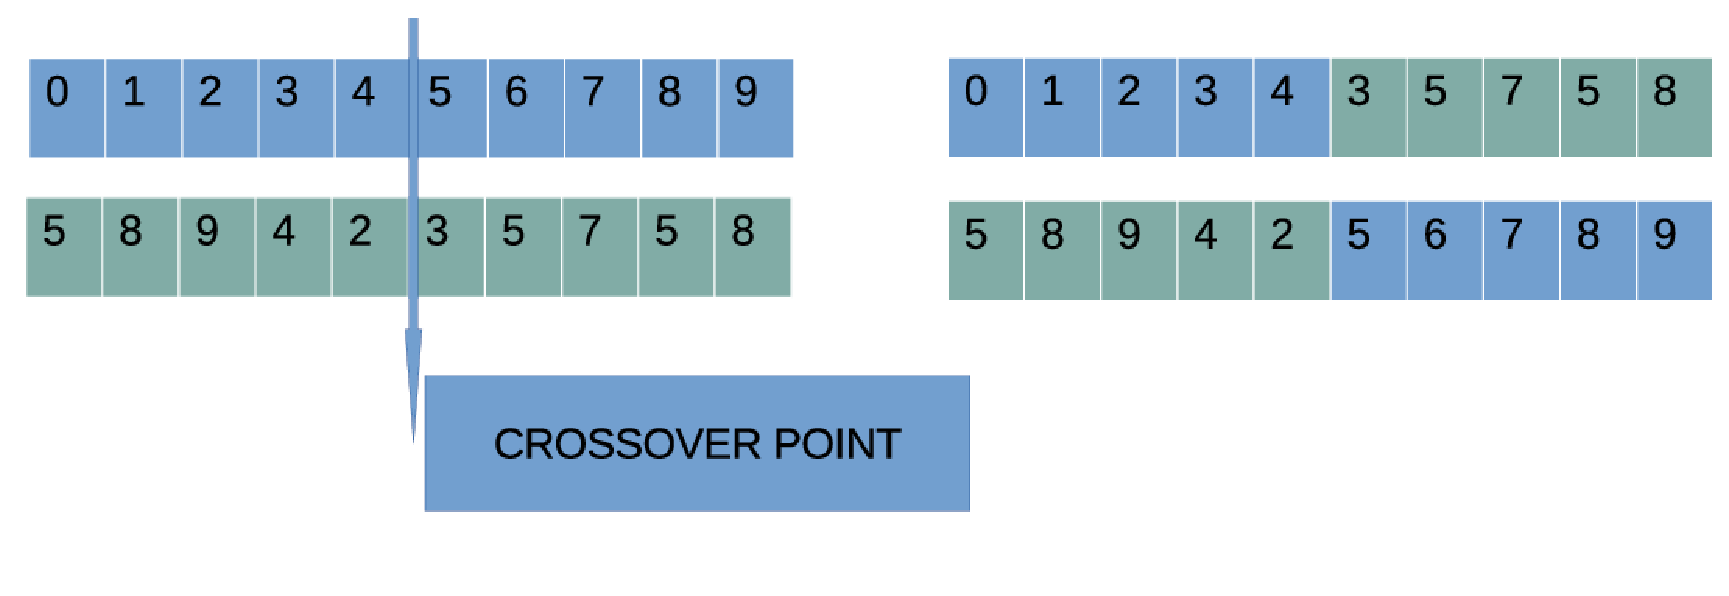
\includegraphics[scale=0.5]{onepoint_crossover}
\par\end{centering}
\caption{An example of the one point crossover procedure, as used in the Grammatical
Evolution.\label{fig:onepoint}}
\end{figure}


\subsection{The second phase of the proposed algorithm}

The second phase utilizes a genetic algorithm, to optimize the parameters
of the RBF network. The optimization of the parameters uses as bounds
the best interval produced in the first phase of the method. The layout
of each chromosome is shown in Figure \ref{fig:The-layout-of}.

\begin{figure}[H]
\caption{The layout of chromosomes in the second phase of the proposed algorithm.\label{fig:The-layout-of}}

$ $
\centering{}{\footnotesize{}}%
\begin{tabular}{|c|c|c|c|c|c|c|c|c|c|c|c|c|c|c|c|c|c|c|c|}
\hline 
{\footnotesize{}$c_{11}$} & {\footnotesize{}$c_{12}$} & {\footnotesize{}...} & {\footnotesize{}$c_{1d}$} & {\footnotesize{}$\sigma_{1}$} & {\footnotesize{}$c_{21}$} & {\footnotesize{}$c_{22}$} & {\footnotesize{}...} & {\footnotesize{}$c_{2d}$} & {\footnotesize{}$\sigma_{2}$} & {\footnotesize{}...} & {\footnotesize{}$c_{k1}$} & {\footnotesize{}$c_{k2}$} & {\footnotesize{}...} & {\footnotesize{}$c_{kd}$} & {\footnotesize{}$\sigma_{k}$} & {\footnotesize{}$w_{1}$} & {\footnotesize{}$w_{2}$} & {\footnotesize{}$\ldots$} & {\footnotesize{}$w_{k}$}\tabularnewline
\hline 
\end{tabular}{\footnotesize\par}
\end{figure}

\begin{enumerate}
\item \textbf{Initialization Step}
\begin{enumerate}
\item \textbf{Define }as $N_{c}$ as the number of chromosomes.
\item \textbf{Define }as $N_{g}$ the total number of generations.
\item \textbf{Define }as $k$ the number of processing nodes of the used
RBF model.
\item \textbf{Define }as $S=\left[L_{\mbox{best}},R_{\mbox{best}}\right]$
the best located interval of the first stage of the algorithm, of
subsection \ref{subsec:The-first-phase}.
\item \textbf{Produce} $N_{C}$ random chromosomes in $S$. 
\item \textbf{Define }as $p_{s}$ the used selection rate, with $p_{s}\le1$.
\item \textbf{Define }as $p_{m}$ the used mutation rate, with $p_{m}\le1$.
\item \textbf{Set} iter=0.
\end{enumerate}
\item \textbf{Fitness calculation Step \label{enu:Fitness-calculation-Step}}
\begin{enumerate}
\item \textbf{For} $i=1,\ldots,N_{g}$ \textbf{do}
\begin{enumerate}
\item \textbf{Compute} the fitness $f_{i}$ of each chromosome $g_{i}$
as $f_{i}=\sum_{j=1}^{m}\left(y\left(\overrightarrow{x_{j}},\overrightarrow{g_{i}}\right)-t_{j}\right)^{2}$
\end{enumerate}
\item \textbf{EndFor}
\end{enumerate}
\item \textbf{Genetic operations step}
\begin{enumerate}
\item \textbf{Selection procedure.} Firstly, sort the chromosomes according
to their fitness values. The first $\left(1-p_{s}\right)\times N_{c}$
chromosomes having the lowest fitness values are copied without changes
to the next generation. The rest of chromosomes are replaced by chromosomes
created in the crossover procedure.
\item \textbf{Crossover procedure}: For every pair of created offsprings
two parents $(z,w)$ are selected from the curent population using
the tournament selection. These parent will produce the offsprings
$\tilde{z}$ and $\tilde{w}$ according to the equations:
\begin{eqnarray}
\tilde{z_{i}} & = & a_{i}z_{i}+\left(1-a_{i}\right)w_{i}\nonumber \\
\tilde{w_{i}} & = & a_{i}w_{i}+\left(1-a_{i}\right)z_{i}\label{eq:crossover_ali-1}
\end{eqnarray}
The value $a_{i}$ is a random number, where $a_{i}\in[-0.5,1.5]$
\citep{kaelo}. 
\item \textbf{Perform} the mutation procedure. In this process a random
number $r\in\left[0,1\right]$ is drawn for every element of each
chromosome. The corresponding element is changed randomly if $r\le p_{m}$.
\end{enumerate}
\item \textbf{Termination Check Step}
\begin{enumerate}
\item \textbf{Set} $iter=iter+1$ 
\item \textbf{If} $\mbox{iter\ensuremath{\le N_{g}} }$goto step \ref{enu:Fitness-calculation-Step}.
\end{enumerate}
%
\end{enumerate}
The steps of the current algorithm are also outlined graphically in
Figure \ref{fig:The-flowchart-of} using a flowchart.

\begin{figure}[H]
\begin{centering}
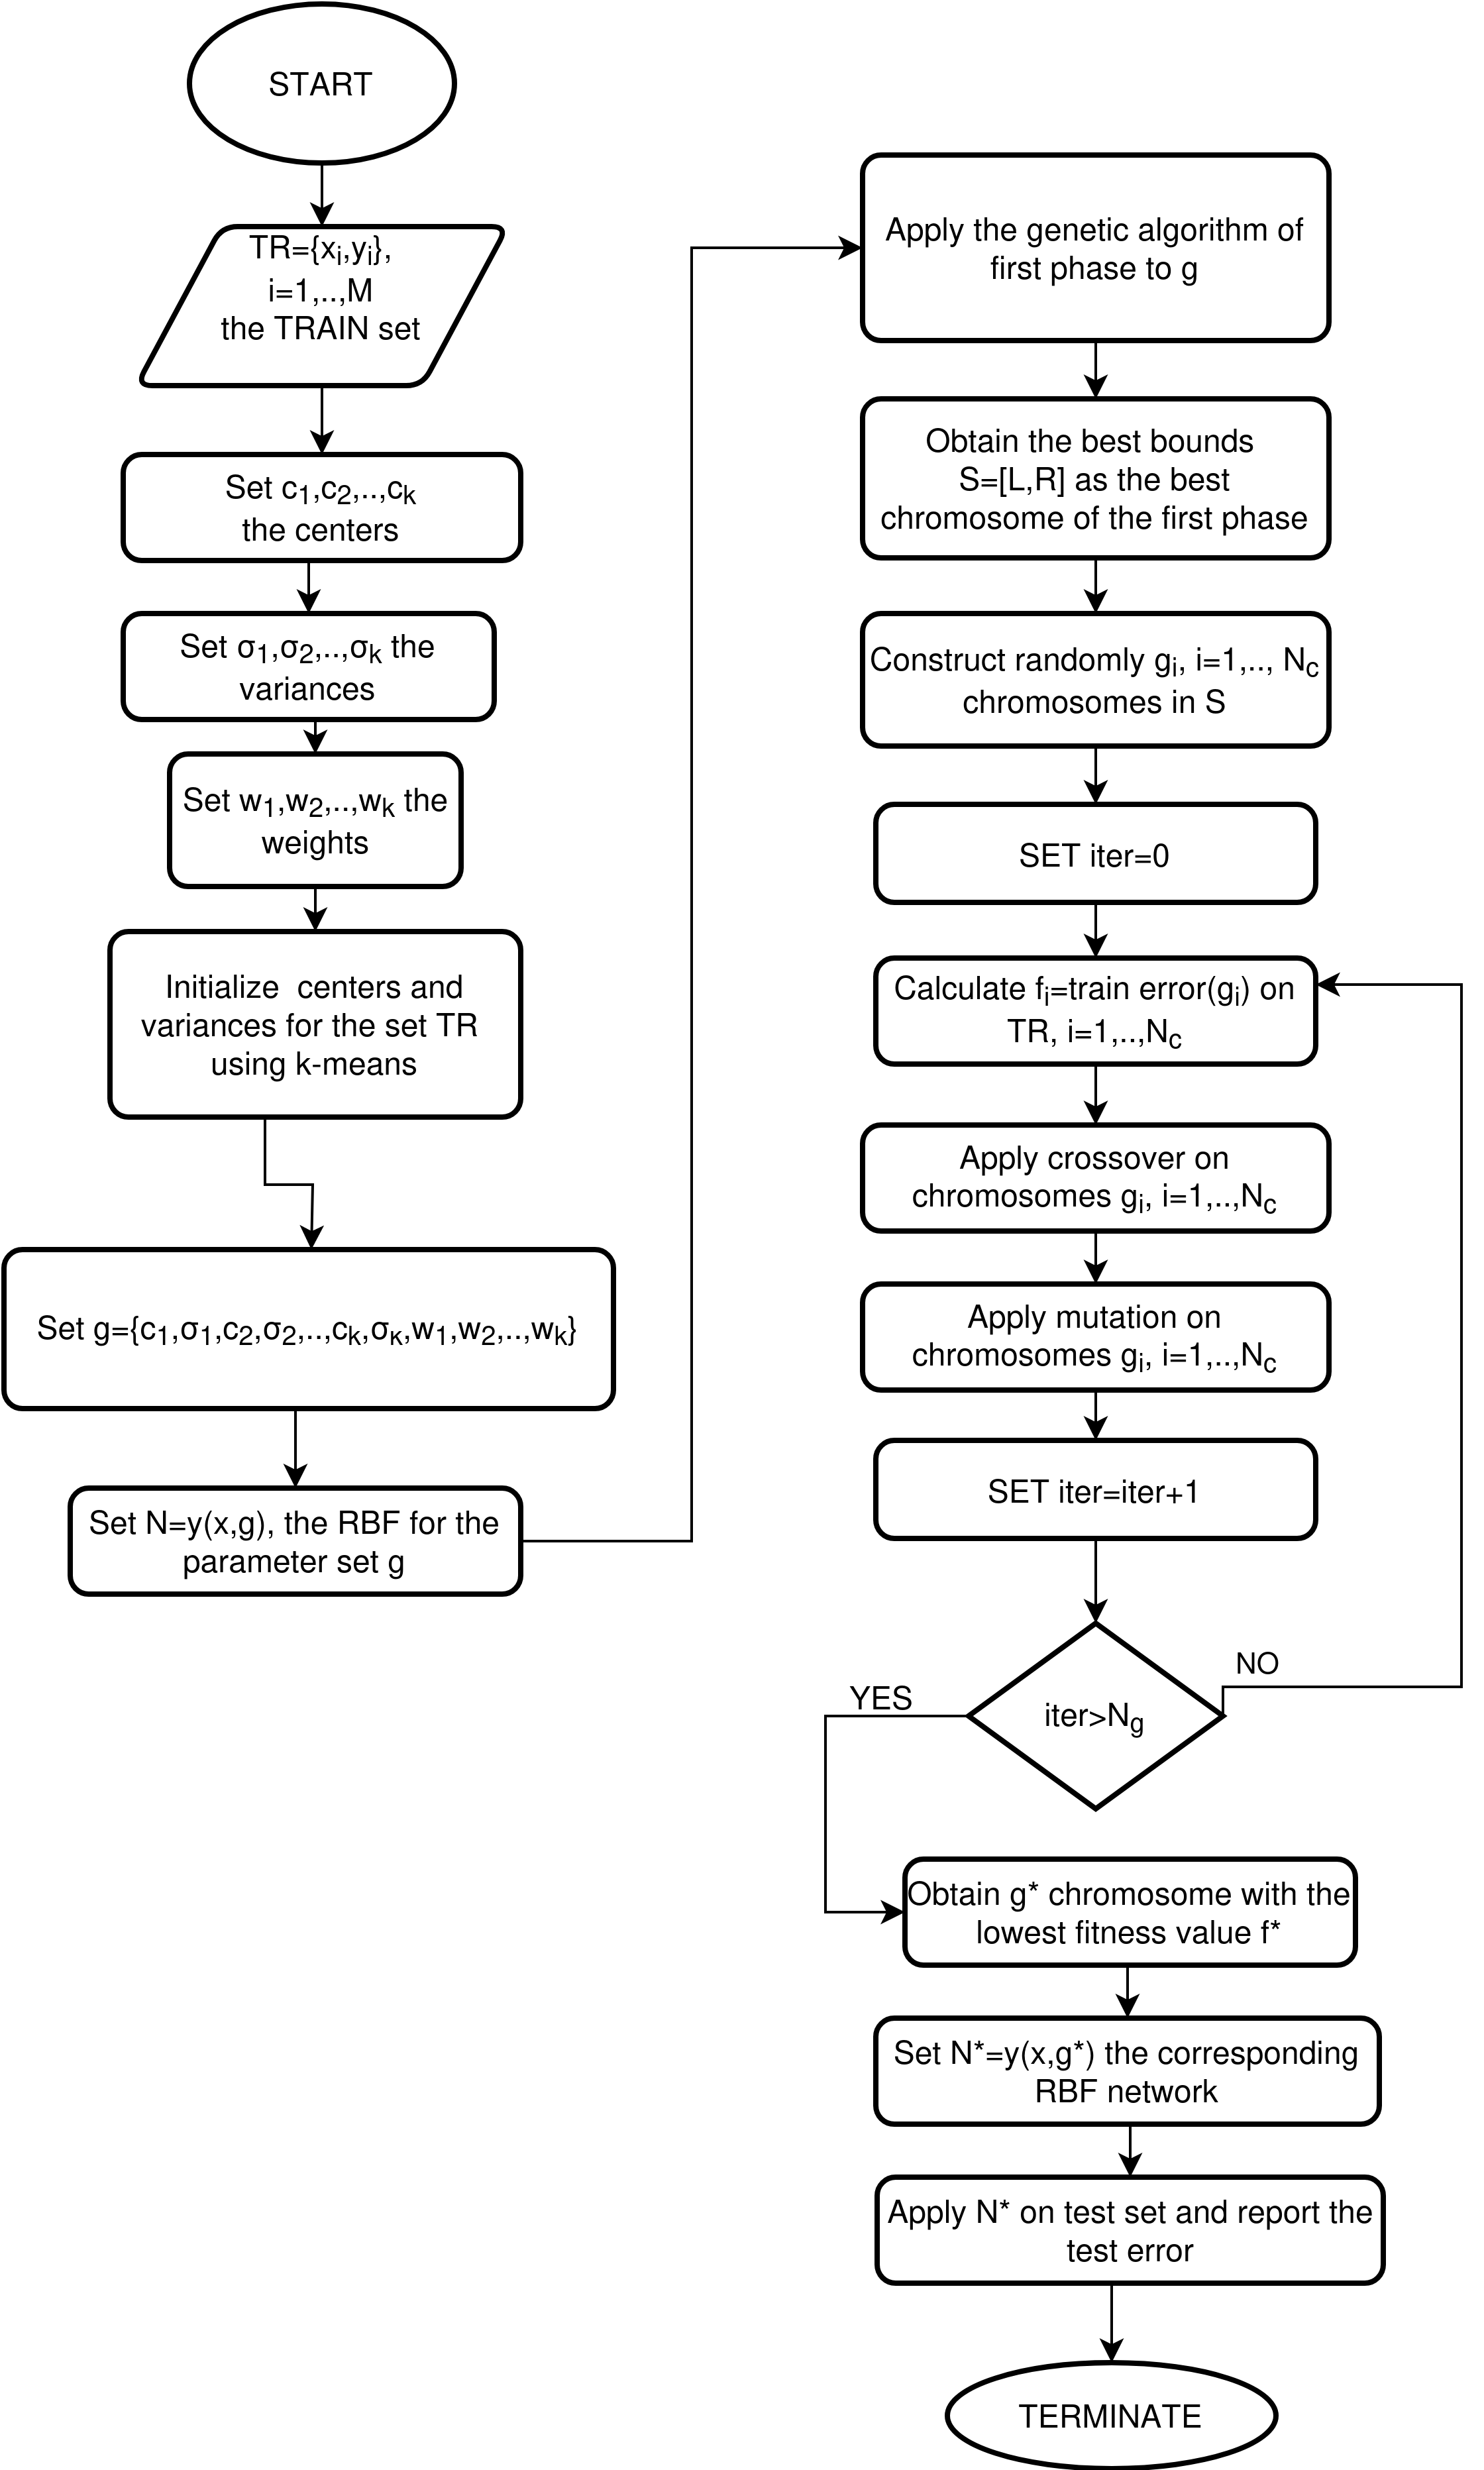
\includegraphics[scale=0.45]{flow}
\par\end{centering}
\caption{The flowchart of the proposed algorithm.\label{fig:The-flowchart-of}}
\end{figure}


\section{Experiments\label{sec:Experiments}}

\subsection{Experimental datasets}

The proposed method was tested on a wide set of classification and
regression problems found in the relevant literature. The method was
compared against some other well -known machine learning models. The
following databases were used to obtain the datasets:
\begin{enumerate}
\item The UCI dataset repository, \url{https://archive.ics.uci.edu/ml/index.php}(accessed
on 9 September 2023)
\item The Keel repository, \url{https://sci2s.ugr.es/keel/datasets.php}(accessed
on 9 September 2023)\citep{Keel}.
\item The Statlib URL \url{http://lib.stat.cmu.edu/datasets/ }(accessed
on 9 September 2023). 
\end{enumerate}
The classification datasets are listed in Table \ref{tab:The-classification-datasets}
and the regression datasets are listed in Table \ref{tab:The-regression-datasets}.

\begin{table}[H]
\caption{The classification datasets used in the experiments. The column DATASET
denotes the number of the dataset, the column CLASSES stands for the
number of classes in each dataset and the column REFERENCE points
to the bibliography where the use of the particular data set is presented.\label{tab:The-classification-datasets}}

\centering{}%
\begin{tabular}{|c|c|c|}
\hline 
DATASET & CLASSES & REFERENCE\tabularnewline
\hline 
\hline 
APPENDICITIS & 2 & \citep{appendicitis}\tabularnewline
\hline 
AUSTRALIAN & 2 & \citep{australian}\tabularnewline
\hline 
BALANCE & 3 & \citep{balance}\tabularnewline
\hline 
CLEVELAND & 5 & \citep{cleveland1,cleveland2}\tabularnewline
\hline 
DERMATOLOGY & 6 & \citep{dermatology}\tabularnewline
\hline 
HAYES ROTH & 3 & \citep{hayesroth}\tabularnewline
\hline 
HEART & 2 & \citep{heart}\tabularnewline
\hline 
HOUSEVOTES & 2 & \citep{housevotes}\tabularnewline
\hline 
IONOSPHERE & 2 & \citep{ion1,ion2}\tabularnewline
\hline 
LIVERDISORDER & 2 & \citep{liver}\tabularnewline
\hline 
MAMMOGRAPHIC & 2 & \citep{mammographic}\tabularnewline
\hline 
PARKINSONS & 2 & \citep{parkinsons}\tabularnewline
\hline 
PIMA & 2 & \citep{pima}\tabularnewline
\hline 
POPFAILURES & 2 & \citep{popfailures}\tabularnewline
\hline 
SPIRAL & 2 & \citep{spiral}\tabularnewline
\hline 
REGIONS2 & 5 & \citep{regions}\tabularnewline
\hline 
SAHEART & 2 & \citep{saheart}\tabularnewline
\hline 
SEGMENT & 7 & \citep{segment}\tabularnewline
\hline 
WDBC & 2 & \citep{wdbc}\tabularnewline
\hline 
WINE & 3 & \citep{wine1,wine2}\tabularnewline
\hline 
Z\_F\_S & 3 & \citep{eeg}\tabularnewline
\hline 
ZO\_NF\_S & 3 & \citep{eeg}\tabularnewline
\hline 
ZONF\_S & 2 & \citep{eeg}\tabularnewline
\hline 
ZOO & 7 & \citep{zoo}\tabularnewline
\hline 
\end{tabular}
\end{table}
\begin{table}[H]
\caption{The regression datasets used in the experiments. The column DATASET
denotes the number of the dataset and the column REFERENCE points
to the bibliography or URL (KEEL or STATLIB) where the use of the
particular data set is presented.\label{tab:The-regression-datasets}}

\centering{}%
\begin{tabular}{|c|c|}
\hline 
DATASET & REFERENCE\tabularnewline
\hline 
\hline 
ABALONE & \citep{abalone}\tabularnewline
\hline 
AIRFOIL & \citep{airfoil}\tabularnewline
\hline 
BASEBALL & STATLIB\tabularnewline
\hline 
BK & \citep{Stat}\tabularnewline
\hline 
BL & STATLIB\tabularnewline
\hline 
CONCRETE & \citep{concrete}\tabularnewline
\hline 
DEE & KEEL\tabularnewline
\hline 
DIABETES & KEEL\tabularnewline
\hline 
FA & STATLIB\tabularnewline
\hline 
HOUSING & \citep{key23}\tabularnewline
\hline 
MB & \citep{key21}\tabularnewline
\hline 
MORTGAGE & KEEL\tabularnewline
\hline 
NT & \citep{ntdataset}\tabularnewline
\hline 
PY & \citep{pydataset}\tabularnewline
\hline 
QUAKE & \citep{quake}\tabularnewline
\hline 
TREASURY & KEEL\tabularnewline
\hline 
WANKARA & KEEL\tabularnewline
\hline 
\end{tabular}
\end{table}


\subsection{Experimental results}

The RBF model used in the experiments was implemented in ANSI C++
with the assistance of the open source Armadillo library \citep{Armadillo}.
The optimization methods used were also freely available from the
OPTIMUS software, downloaded from \url{https://github.com/itsoulos/OPTIMUS/}(accessed
on 9 September 2023). The proposed method was validated using the
10 - fold validation technique for all datasets. Also, all the experiments
were executed 30 times with different seed number for the random generator
each time. In the conducted experiments, the drand48() random function
of the C - programming language was employed. For the classification
datasets the average classification error was measured and and the
average mean test error for the regression datasets. The experiments
were conducted on an AMD Ryzen 5950X with 128GB of RAM, running the
Debian Linux operating system. All the values for the parameters of
the used algorithms are shown in Table \ref{tab:Experimental-parameters}.
The results obtained for the classification datasets are shown in
Table \ref{tab:Experiments-for-classification} and for the regression
datasets are listed in Table \ref{tab:experiments-regression}. 

The following applies to the results tables:
\begin{enumerate}
\item The column RPROP represents an artificial neural network \citep{nn1,nn2}.
This neural network has 10 processing nodes and was trained using
the Rprop method \citep{rpropnn}.
\item The column denoted as ADAM stands for an artificial neural network
with 10 hidden nodes trained by the Adam optimizer \citep{Adam,AdamNN}.
\item The column NEAT (NeuroEvolution of Augmenting Topologies ) \citep{neat}
denotes the application of the NEAT method for neural network training.
\item The RBF-KMEANS column denotes the original two - phase training method
for RBF networks. During the first phase the centers and variances
are estimated through the K-Means algorithm and during the second
phase the output weights are calculated by solving a linear system
of equations.
\item The column GENRBF stands for the RBF training method introduced in
\citep{rbf_gen1}.
\item The column PROPOSED represents the results obtained by the proposed
method.
\item For both tables, an additional line was added under the title AVERAGE.
This line indicates the average classification or regression error
for all datasets.
\end{enumerate}
\begin{table}[H]
\caption{The values used for the experimental parameters.\label{tab:Experimental-parameters}}

\centering{}%
\begin{tabular}{|c|c|}
\hline 
\textbf{PARAMETER} & \textbf{VALUE}\tabularnewline
\hline 
$N_{c}$ & 200\tabularnewline
\hline 
$N_{g}$ & 100\tabularnewline
\hline 
$N_{s}$ & 50\tabularnewline
\hline 
$F$ & 10.0\tabularnewline
\hline 
$B$ & 100.0\tabularnewline
\hline 
$k$ & 10\tabularnewline
\hline 
$p_{s}$ & 0.90\tabularnewline
\hline 
$p_{m}$ & 0.05\tabularnewline
\hline 
\end{tabular}
\end{table}

\begin{table}[H]
\caption{Experimental results for the classification datasets. The first column
denotes the name of the dataset. Every number in cells denote average
classification error as calculated on the test set.\label{tab:Experiments-for-classification}}

\centering{}%
\begin{tabular}{|c|c|c|c|c|c|c|}
\hline 
\textbf{DATASET} & \textbf{RPROP} & \textbf{ADAM} & \textbf{NEAT} & \textbf{RBF-KMEANS} & \textbf{GENRBF} & \textbf{PROPOSED}\tabularnewline
\hline 
\hline 
Appendicitis & 16.30\% & 16.50\% & 17.20\% & 12.23\% & 16.83\% & 15.77\%\tabularnewline
\hline 
Australian & 36.12\% & 35.65\% & 31.98\% & 34.89\% & 41.79\% & 22.40\%\tabularnewline
\hline 
Balance & 8.81\% & 7.87\% & 23.14\% & 33.42\% & 38.02\% & 15.62\%\tabularnewline
\hline 
Cleveland & 61.41\% & 67.55\% & 53.44\% & 67.10\% & 67.47\% & 50.37\%\tabularnewline
\hline 
Dermatology & 15.12\% & 26.14\% & 32.43\% & 62.34\% & 61.46\% & 35.73\%\tabularnewline
\hline 
Hayes Roth & 37.46\% & 59.70\% & 50.15\% & 64.36\% & 63.46\% & 35.33\%\tabularnewline
\hline 
Heart & 30.51\% & 38.53\% & 39.27\% & 31.20\% & 28.44\% & 15.91\%\tabularnewline
\hline 
HouseVotes & 6.04\% & 7.48\% & 10.89\% & 6.13\% & 11.99\% & 3.33\%\tabularnewline
\hline 
Ionosphere & 13.65\% & 16.64\% & 19.67\% & 16.22\% & 19.83\% & 9.30\%\tabularnewline
\hline 
Liverdisorder & 40.26\% & 41.53\% & 30.67\% & 30.84\% & 36.97\% & 28.44\%\tabularnewline
\hline 
Mammographic & 18.46\% & 46.25\% & 22.85\% & 21.38\% & 30.41\% & 17.72\%\tabularnewline
\hline 
Parkinsons & 22.28\% & 24.06\% & 18.56\% & 17.41\% & 33.81\% & 14.53\%\tabularnewline
\hline 
Pima & 34.27\% & 34.85\% & 34.51\% & 25.78\% & 27.83\% & 23.33\%\tabularnewline
\hline 
Popfailures & 4.81\% & 5.18\% & 7.05\% & 7.04\% & 7.08\% & 4.68\%\tabularnewline
\hline 
Regions2 & 27.53\% & 29.85\% & 33.23\% & 38.29\% & 39.98\% & 25.18\%\tabularnewline
\hline 
Saheart & 34.90\% & 34.04\% & 34.51\% & 32.19\% & 33.90\% & 29.46\%\tabularnewline
\hline 
Segment & 52.14\% & 49.75\% & 66.72\% & 59.68\% & 54.25\% & 49.22\%\tabularnewline
\hline 
Spiral & 46.59\% & 48.90\% & 50.22\% & 44.87\% & 50.02\% & 23.58\%\tabularnewline
\hline 
Wdbc & 21.57\% & 35.35\% & 12.88\% & 7.27\% & 8.82\% & 5.20\%\tabularnewline
\hline 
Wine & 30.73\% & 29.40\% & 25.43\% & 31.41\% & 31.47\% & 5.63\%\tabularnewline
\hline 
Z\_F\_S & 29.28\% & 47.81\% & 38.41\% & 13.16\% & 23.37\% & 3.90\%\tabularnewline
\hline 
ZO\_NF\_S & 6.43\% & 47.43\% & 43.75\% & 9.02\% & 22.18\% & 3.99\%\tabularnewline
\hline 
ZONF\_S & 27.27\% & 11.99\% & 5.44\% & 4.03\% & 17.41\% & 1.67\%\tabularnewline
\hline 
ZOO & 15.47\% & 14.13\% & 20.27\% & 21.93\% & 33.50\% & 9.33\%\tabularnewline
\hline 
\textbf{AVERAGE} & \textbf{26.56\%} & \textbf{32.36\%} & \textbf{30.11\%} & \textbf{28.84\%} & \textbf{33.35\%} & \textbf{18.73\%}\tabularnewline
\hline 
\end{tabular}
\end{table}

\begin{table}[H]
\caption{Experimental results for the regression datasets. The first column
is the name of the regression dataset. Also, the numbers in cells
denote average regression error on the test set.\label{tab:experiments-regression}}

\centering{}%
\begin{tabular}{|c|c|c|c|c|c|c|}
\hline 
\textbf{DATASET} & \textbf{RPROP} & \textbf{ADAM} & \textbf{NEAT} & \textbf{RBF-KMEANS} & \textbf{GENRBF} & \textbf{PROPOSED}\tabularnewline
\hline 
ABALONE & 4.55 & 4.30 & 9.88 & 7.37 & 9.98 & 5.16\tabularnewline
\hline 
AIRFOIL & 0.002 & 0.005 & 0.067 & 0.27 & 0.121 & 0.004\tabularnewline
\hline 
BASEBALL & 92.05 & 77.90 & 100.39 & 93.02 & 98.91 & 81.26\tabularnewline
\hline 
BK & 1.60 & 0.03 & 0.15 & 0.02 & 0.023 & 0.025\tabularnewline
\hline 
BL & 4.38 & 0.28 & 0.05 & 0.013 & 0.005 & 0.0004\tabularnewline
\hline 
CONCRETE & 0.009 & 0.078 & 0.081 & 0.011 & 0.015 & 0.006\tabularnewline
\hline 
DEE & 0.608 & 0.630 & 1.512 & 0.17 & 0.25 & 0.16\tabularnewline
\hline 
DIABETES & 1.11 & 3.03 & 4.25 & 0.49 & 2.92 & 1.74\tabularnewline
\hline 
HOUSING & 74.38 & 80.20 & 56.49 & 57.68 & 95.69 & 21.11\tabularnewline
\hline 
FA & 0.14 & 0.11 & 0.19 & 0.015 & 0.15 & 0.033\tabularnewline
\hline 
MB & 0.55 & 0.06 & 0.061 & 2.16 & 0.41 & 0.19\tabularnewline
\hline 
MORTGAGE & 9.19 & 9.24 & 14.11 & 1.45 & 1.92 & 0.014\tabularnewline
\hline 
NT & 0.04 & 0.12 & 0.33 & 8.14 & 0.02 & 0.007\tabularnewline
\hline 
PY & 0.039 & 0.09 & 0.075 & 0.012 & 0.029 & 0.019\tabularnewline
\hline 
QUAKE & 0.041 & 0.06 & 0.298 & 0.07 & 0.79 & 0.034\tabularnewline
\hline 
TREASURY & 10.88 & 11.16 & 15.52 & 2.02 & 1.89 & 0.098\tabularnewline
\hline 
WANKARA & 0.0003 & 0.02 & 0.005 & 0.001 & 0.002 & 0.003\tabularnewline
\hline 
\textbf{AVERAGE} & \textbf{11.71} & \textbf{11.02} & \textbf{11.97} & \textbf{10.17} & \textbf{12.54} & \textbf{6.46}\tabularnewline
\hline 
\end{tabular}
\end{table}

On average, the proposed technique appears to be 30-40\% more accurate
than the immediate best. In many cases, this percentage exceeds 70\%.
Moreover, in the vast majority of problems, the proposed technique
significantly outperforms the next best available method in terms
of test error. In order to validate the results, an additional experiment
was executed on the classification datasets, where the number of nodes
increases from 5 to 20 and the results are graphically outlined in
Figure \ref{fig:nodesExperiment}. From this experiment, one can draw
two conclusions: firstly, the proposed technique has a significant
advantage over the others to a large extent in terms of average classification
error, and secondly, the proposed method is shown to be robust and
not significantly dependent on the increase of processing nodes ,
since 5--10 processing nodes are enough to achieve low classification
errors.

\begin{figure}[H]
\begin{centering}
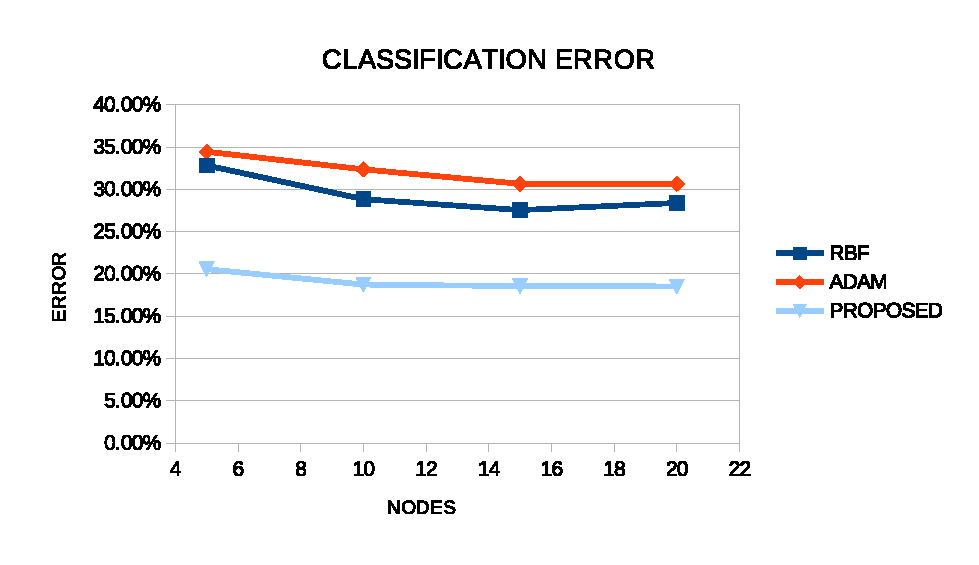
\includegraphics[scale=0.6]{nodes_plot}
\par\end{centering}
\caption{Average classification error for all classification datasets. The
number of nodes increases from 5 to 20 and three models were used:
the ADAM optimizer to optimize a neural network, the original RBF
training method of two phases and the proposed method.\label{fig:nodesExperiment}}

\end{figure}

However, the proposed technique consists of two stages and in each
of them a genetic algorithm should be executed. This means that it
is significantly slower in computing time compared to the rest of
the techniques and, of course, it needs more computing resources.
This is graphically shown in Figure \ref{fig:timeExperiment}, where
the average execution time for the method ADAM and the proposed method
is shown for the classification datasets, when the number of processing
nodes increases from 5 to 20. As expected, the proposed technique
requires significantly more time than a traditional neural network
training technique such as ADAM, since it consists of two sequential
genetic algorithms.

\begin{figure}[H]
\begin{centering}
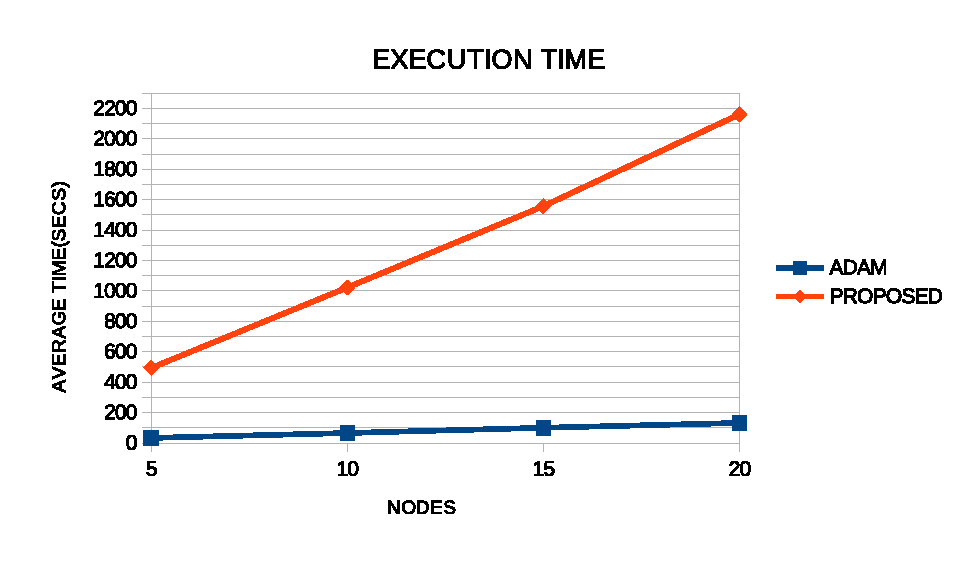
\includegraphics[scale=0.6]{time_plot}
\par\end{centering}
\caption{Average execution time for the ADAM method used to train a neural
network and the proposed technique.\label{fig:timeExperiment}}

\end{figure}

Of course, since we are talking about Genetic Algorithms, the training
time required could be significantly reduced by using parallel techniques
that take advantage of modern parallel computing structures such as
the MPI interface \citep{openmpi} or the OpenMP library \citep{openmp}.
The superiority of the proposed technique is also reinforced by the
statistical tests carried out on the experimental results and presented
in figure \ref{fig:statClass}.

\begin{figure}[H]
\begin{centering}
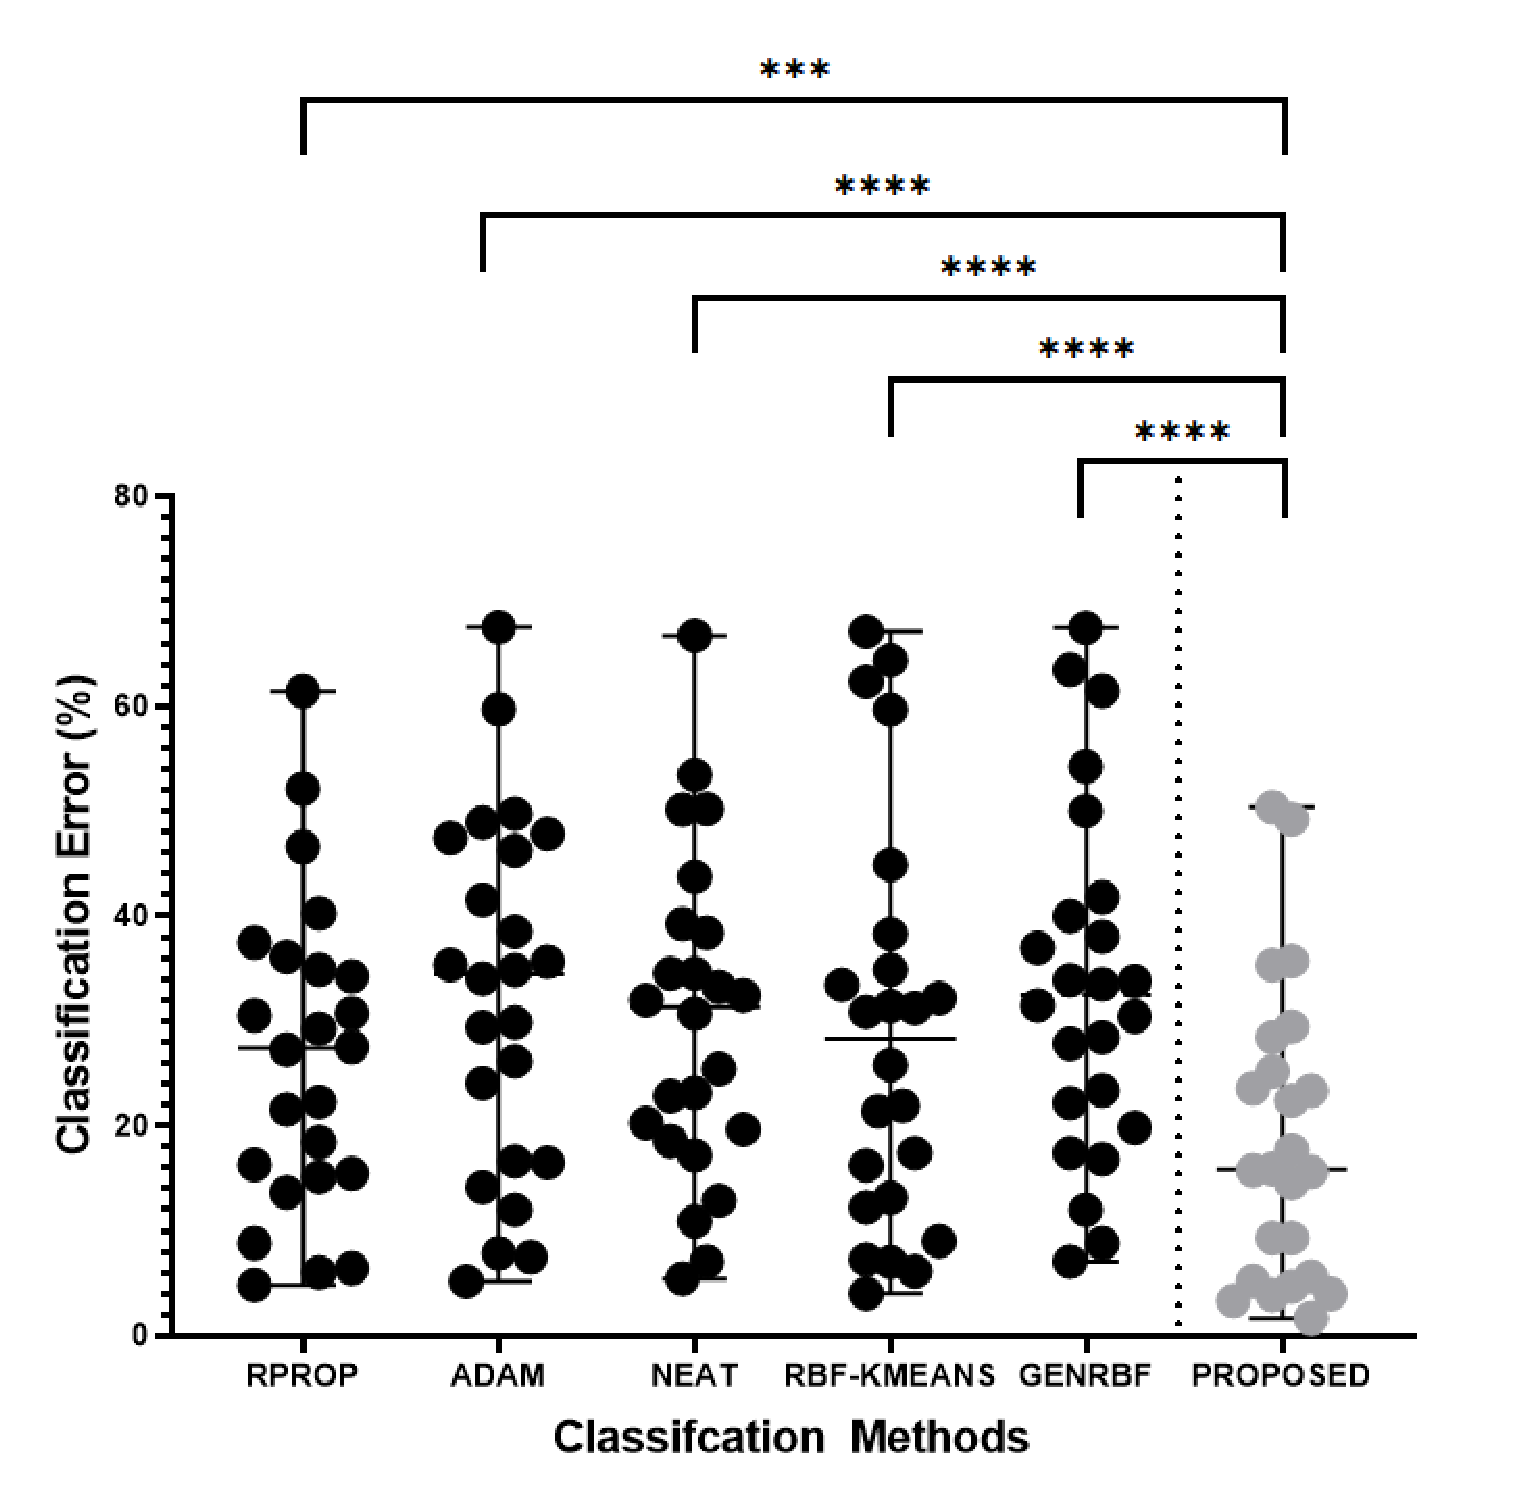
\includegraphics[scale=0.4]{stat_class_genrbf}
\par\end{centering}
\caption{Scatter plot representation and the two-sample paired (Wilcoxon) signed-rank
test results of the comparison for each of the five (5) classification
methods (RPROP, ADAM, NEAT, RBF-KMEANS, and GENRBF) with the PROPOSED
method regarding the classification error in twenty-four (24) different
public available classification datasets. The stars only intend to
flag significance levels for the two most used groups. A p-value of
less than 0.001 is flagged with three stars ({*}{*}). A p-value of
less than 0.0001 is flagged with four stars ({*}{*}{*}).\label{fig:statClass}}
\end{figure}
 

In addition, an additional set of experiments was performed on the
classification data in which the critical parameter $F$ took the
values 3, 5 and 10. The aim of this set of experiments was to establish
the sensitivity of the proposed technique to changes in its parameters.
The experimental results are presented in the table \ref{tab:expsFClass}
and a statistical test on the results is presented in figure \ref{fig:statfparam}.
The results and the statistics test indicate that there is no significant
difference in the efficiency of the method for different values of
the critical parameter $F$.

\begin{table}[H]
\caption{Experimental results with the proposed method and using different
values for the parameter $F$ on the classification datasets.\label{tab:expsFClass}}

\centering{}%
\begin{tabular}{|c|c|c|c|}
\hline 
\textbf{DATASET} & \textbf{$F=3$} & \textbf{$F=5$} & \textbf{$F=10$}\tabularnewline
\hline 
Appendicitis & 15.57\% & 16.60\% & 15.77\%\tabularnewline
\hline 
Australian & 24.29\% & 23.94\% & 22.40\%\tabularnewline
\hline 
Balance & 17.22\% & 15.39\% & 15.62\%\tabularnewline
\hline 
Cleveland & 52.09\% & 51.65\% & 50.37\%\tabularnewline
\hline 
Dermatology & 37.23\% & 36.81\% & 35.73\%\tabularnewline
\hline 
Hayes Roth & 35.72\% & 32.31\% & 35.33\%\tabularnewline
\hline 
Heart & 16.32\% & 15.54\% & 15.91\%\tabularnewline
\hline 
HouseVotes & 4.35\% & 3.90\% & 3.33\%\tabularnewline
\hline 
Ionosphere & 12.50\% & 11.44\% & 9.30\%\tabularnewline
\hline 
Liverdisorder & 28.08\% & 28.19\% & 28.44\%\tabularnewline
\hline 
Mammographic & 17.49\% & 17.15\% & 17.72\%\tabularnewline
\hline 
Parkinsons & 16.25\% & 15.17\% & 14.53\%\tabularnewline
\hline 
Pima & 23.29\% & 23.97\% & 23.33\%\tabularnewline
\hline 
Popfailures & 5.31\% & 5.86\% & 4.68\%\tabularnewline
\hline 
Regions2 & 25.97\% & 26.29\% & 25.18\%\tabularnewline
\hline 
Saheart & 28.52\% & 28.59\% & 29.46\%\tabularnewline
\hline 
Segment & 44.95\% & 48.77\% & 49.22\%\tabularnewline
\hline 
Spiral & 15.49\% & 18.19\% & 23.58\%\tabularnewline
\hline 
Wdbc & 5.43\% & 5.01\% & 5.20\%\tabularnewline
\hline 
Wine & 7.59\% & 8.39\% & 5.63\%\tabularnewline
\hline 
Z\_F\_S & 4.37\% & 4.26\% & 3.90\%\tabularnewline
\hline 
ZO\_NF\_S & 3.79\% & 4.21\% & 3.99\%\tabularnewline
\hline 
ZONF\_S & 2.34\% & 2.26\% & 1.67\%\tabularnewline
\hline 
ZOO & 11.90\% & 10.50\% & 9.33\%\tabularnewline
\hline 
\textbf{AVERAGE} & \textbf{19.03\%} & \textbf{18.93\%} & \textbf{18.73\%}\tabularnewline
\hline 
\end{tabular}
\end{table}
\begin{figure}[H]
\begin{centering}
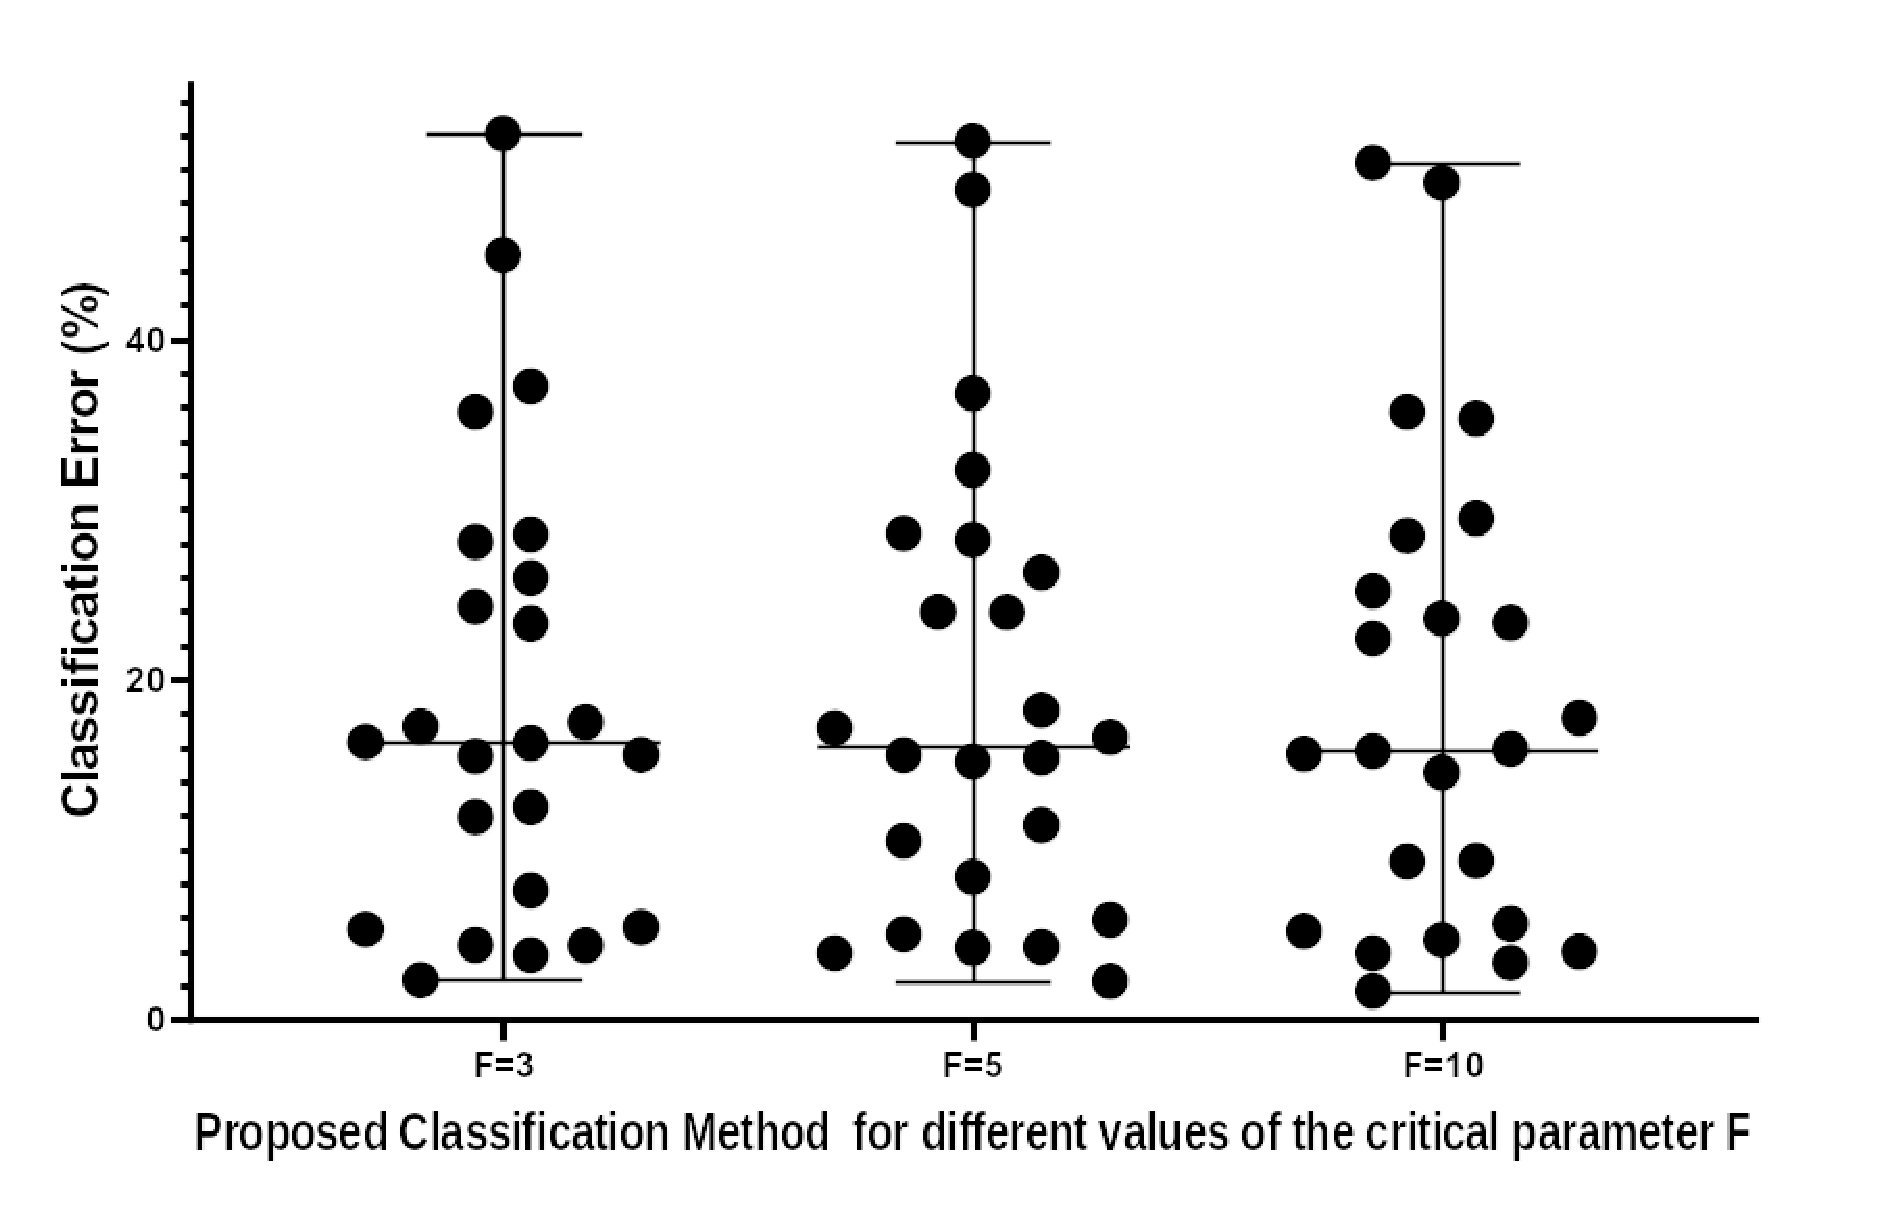
\includegraphics[scale=0.4]{stat_fparam_genrbf}
\par\end{centering}
\caption{A Friedman test was conducted to determine whether different values
of the critical parameter F had a difference or not in the classification
error of the proposed method in twenty-four (24) other publicly available
classification datasets. The analysis results for three different
values of the critical parameter F (F=3, F=5, F=10) indicated no significant
difference.\label{fig:statfparam}}
\end{figure}


\section{Conclusions}

In the current work, an innovative two-stage technique was proposed
for efficient training of RBF artificial neural networks. In the first
stage of the application, using Grammatical Evolution, the interval
of values of the neural network parameters is partitioned, so as to
find a promising range that may contain low values of the training
error. In the second stage, the neural network parameters are trained
within the best range of values found in the first stage. The training
of the parameters of the second phase is carried out using a Genetic
Algorithm. The proposed method was applied on a wide series of well
-known datasets from the relevant literature and was tested against
a series of machine learning models. The new training technique was
compared with the traditional method of training RBF networks but
also with other training techniques of machine learning models and
from the experimental results its superiority is evident in percentages
that exceed 40\%. However, since the proposed technique consists of
two genetic algorithms executed sequentially, the execution time required
is longer compared to other techniques especially for datasets with
many patterns. An immediate solution to reduce the execution time
of the method would be the use of parallel computing techniques, since
genetic algorithms can by nature be directly parallelized.

Future improvements to the proposed method may include:
\begin{enumerate}
\item Application of the proposed method to other types of artificial neural
networks.
\item Use of intelligent learning techniques in place of the K-Means technique
to initialize the neural network parameters.
\item Using techniques to dynamically determine the number of necessary
parameters of the neural network. For the time being, the number of
parameters is considered constant, but this has the consequence of
observing over-training phenomena in various data sets.
\item Implementation of crossover and mutation techniques that focus more
on the existing interval construction technique for the model parameters.
\item Use of efficient termination techniques for Genetic Algorithms, for
the most efficient termination of techniques without wasting computing
time on unnecessary iterations.
\item Incorporation of parallel programming techniques to speed up the method.
\end{enumerate}
\vspace{6pt}

$ $

\authorcontributions{I.G.T., A.T. and E.K. conceived the idea and methodology and supervised
the technical part regarding the software. I.G.T. executed the experiments,
employing several datasets. A.T. performed the statistical analysis
and all authors prepared the manuscript. All authors have read and
agreed to the published version of the manuscript.}

\funding{This research received no external funding.}

\institutionalreview{Not applicable.}

\informedconsent{Not applicable.}

\dataavailability{Not applicable.}

\acknowledgments{This research has been financed by the European Union : Next Generation
EU through the Program Greece 2.0 National Recovery and Resilience
Plan , under the call RESEARCH -- CREATE -- INNOVATE, project name
“iCREW: Intelligent small craft simulator for advanced crew training
using Virtual Reality techniques\textquotedbl{} (project code:TAEDK-06195)}

\conflictsofinterest{The authors declare no conflict of interest.}

\appendixtitles{no}

\appendixstart{}

\appendix

\begin{adjustwidth}{-\extralength}{0cm}{}


\reftitle{References}
\begin{thebibliography}{999}
\bibitem{physics_ml1} M. Mjahed, The use of clustering techniques
for the classification of high energy physics data, Nuclear Instruments
and Methods in Physics Research Section A: Accelerators, Spectrometers,
Detectors and Associated Equipment \textbf{559}, pp. 199-202, 2006.

\bibitem{physics_ml2}M Andrews, M Paulini, S Gleyzer, B Poczos, End-to-End
Event Classification of High-Energy Physics Data, Journal of Physics:
Conference Series \textbf{1085}, 2018.

\bibitem{chemistry_ml1}P. He, C.J. Xu, Y.Z. Liang, K.T. Fang, Improving
the classification accuracy in chemistry via boosting technique, Chemometrics
and Intelligent Laboratory Systems 70, pp. 39-46, 2004.

\bibitem{chemistry_ml2}J.A. Aguiar, M.L. Gong, T.Tasdizen, Crystallographic
prediction from diffraction and chemistry data for higher throughput
classification using machine learning, Computational Materials Science
\textbf{173}, 109409, 2020.

\bibitem{econ_ml1}I. Kaastra, M. Boyd, Designing a neural network
for forecasting financial and economic time series, Neurocomputing
\textbf{10}, pp. 215-236, 1996.

\bibitem{econ_ml2}R. Hafezi, J. Shahrabi, E. Hadavandi, A bat-neural
network multi-agent system (BNNMAS) for stock price prediction: Case
study of DAX stock price, Applied Soft Computing \textbf{29}, pp.
196-210, 2015.

\bibitem{med_ml1}S.S. Yadav, S.M. Jadhav, Deep convolutional neural
network based medical image classification for disease diagnosis.
J Big Data \textbf{6}, 113, 2019.

\bibitem{med_ml2}L. Qing, W. Linhong , D. Xuehai, A Novel Neural
Network-Based Method for Medical Text Classification, Future Internet
\textbf{11}, 255, 2019. 

\bibitem{rbf1}J. Park and I. W. Sandberg, Universal Approximation
Using Radial-Basis-Function Networks, Neural Computation \textbf{3},
pp. 246-257, 1991.

\bibitem{rbf2}G.A. Montazer, D. Giveki, M. Karami, H. Rastegar, Radial
basis function neural networks: A review. Comput. Rev. J \textbf{1},
pp. 52-74, 2018.

\bibitem{nnreview}O.I. Abiodun, A. Jantan, A. E. Omolara, K.V. Dada,
N. A. Mohamed, H. Arshad, State-of-the-art in artificial neural network
applications: A survey, Heliyon \textbf{4}, e00938, 2018.

\bibitem{rbf_approx}Y. Liao, S. C. Fang, and H. L. W. Nuttle, “Relaxed
conditions for radial-basis function networks to be universal approximators,”
Neural Networks, vol. 16, no. 7, pp. 1019--1028, 2003

\bibitem{rbfphysics1}P. Teng, Machine-learning quantum mechanics:
Solving quantum mechanics problems using radial basis function networks,
Phys. Rev. E \textbf{98}, 033305, 2018.

\bibitem{rbfphysics2}R. Jovanović, A. Sretenovic, Ensemble of radial
basis neural networks with K-means clustering for heating energy consumption
prediction, FME Transactions \textbf{45}, pp. 51-57, 2017.

\bibitem{rbfphysics3}V.I. Gorbachenko, M.V. Zhukov, Solving boundary
value problems of mathematical physics using radial basis function
networks. Comput. Math. and Math. Phys. \textbf{57}, pp. 145--155,
2017.

\bibitem{rbfphysics4}J. Määttä, V. Bazaliy, J. Kimari, F. Djurabekova,
K. Nordlund, T. Roos, Gradient-based training and pruning of radial
basis function networks with an application in materials physics,
Neural Networks \textbf{133}, pp. 123-131, 2021.

\bibitem{rbfde1}Nam Mai-Duy, Thanh Tran-Cong, Numerical solution
of differential equations using multiquadric radial basis function
networks, Neural Networks 14, pp. 185-199, 2001.

\bibitem{rbfde2}N. Mai‐Duy, Solving high order ordinary differential
equations with radial basis function networks. Int. J. Numer. Meth.
Engng. \textbf{62}, pp. 824-852, 2005.

\bibitem{rbfde3}S.A. Sarra, Adaptive radial basis function methods
for time dependent partial differential equations, Applied Numerical
Mathematics \textbf{54}, pp. 79-94, 2005.

\bibitem{rbfrobotics1}R. -J. Lian, Adaptive Self-Organizing Fuzzy
Sliding-Mode Radial Basis-Function Neural-Network Controller for Robotic
Systems, IEEE Transactions on Industrial Electronics \textbf{61},
pp. 1493-1503, 2014.

\bibitem{rbfrobotics2}M. Vijay, D. Jena, Backstepping terminal sliding
mode control of robot manipulator using radial basis functional neural
networks. Computers \& Electrical Engineering \textbf{67}, pp. 690-707,
2018.

\bibitem{rbfface1}M.J. Er, S. Wu, J. Lu, H.L. Toh, Face recognition
with radial basis function (RBF) neural networks, IEEE Transactions
on Neural Networks \textbf{13}, pp. 697-710, 2002.

\bibitem{rbfnetwork1}C. Laoudias, P. Kemppi and C. G. Panayiotou,
Localization Using Radial Basis Function Networks and Signal Strength
Fingerprints in WLAN, GLOBECOM 2009 - 2009 IEEE Global Telecommunications
Conference, Honolulu, HI, 2009, pp. 1-6, 2009.

\bibitem{rbfnetwork2}M. Azarbad, S. Hakimi, A. Ebrahimzadeh, Automatic
recognition of digital communication signal, International journal
of energy, information and communications \textbf{3}, pp. 21-33, 2012.

\bibitem{rbfchemistry1}D.L. Yu, J.B. Gomm, D. Williams, Sensor fault
diagnosis in a chemical process via RBF neural networks, Control Engineering
Practice \textbf{7}, pp. 49-55, 1999.

\bibitem{rbfchemistry2}V. Shankar, G.B. Wright, A.L. Fogelson, R.M.
Kirby, A radial basis function (RBF) finite difference method for
the simulation of reaction--diffusion equations on stationary platelets
within the augmented forcing method, Int. J. Numer. Meth. Fluids \textbf{75},
pp. 1-22, 2014.

\bibitem{rbfecon0}W. Shen, X. Guo, C. Wu, D. Wu, Forecasting stock
indices using radial basis function neural networks optimized by artificial
fish swarm algorithm, Knowledge-Based Systems 24, pp. 378-385, 2011.

\bibitem{rbfecon1}J. A. Momoh, S. S. Reddy, Combined Economic and
Emission Dispatch using Radial Basis Function, 2014 IEEE PES General
Meeting \textbar{} Conference \& Exposition, National Harbor, MD,
pp. 1-5, 2014.

\bibitem{rbfecon2}P. Sohrabi, B. Jodeiri Shokri, H. Dehghani, Predicting
coal price using time series methods and combination of radial basis
function (RBF) neural network with time series. Miner Econ 2021.

\bibitem{rbf_dos1}U. Ravale, N. Marathe, P. Padiya, Feature Selection
Based Hybrid Anomaly Intrusion Detection System Using K Means and
RBF Kernel Function, Procedia Computer Science \textbf{45}, pp. 428-435,
2015.

\bibitem{rbf_dos2}M. Lopez-Martin, A. Sanchez-Esguevillas, J. I.
Arribas, B. Carro, Network Intrusion Detection Based on Extended RBF
Neural Network With Offline Reinforcement Learning, IEEE Access \textbf{9},
pp. 153153-153170, 2021.

\bibitem{rbfinit1}L.I. Kuncheva, Initializing of an RBF network by
a genetic algorithm, Neurocomputing \textbf{14}, pp. 273-288, 1997.

\bibitem{rbfinit2}F. Ros, M. Pintore, A. Deman, J.R. Chrétien, Automatical
initialization of RBF neural networks, Chemometrics and Intelligent
Laboratory Systems \textbf{87}, pp. 26-32, 2007.

\bibitem{rbfinit3}D. Wang, X.J. Zeng, J.A. Keane, A clustering algorithm
for radial basis function neural network initialization, Neurocomputing
\textbf{77}, pp. 144-155, 2012.

\bibitem{rbfkernel}N. Benoudjit, M. Verleysen, On the Kernel Widths
in Radial-Basis Function Networks, Neural Processing Letters \textbf{18},
pp. 139--154, 2003.

\bibitem{rbflearn}R. Neruda, P. Kudova, Learning methods for radial
basis function networks, Future Generation Computer Systems \textbf{21},
pp. 1131--1142, 2005.

\bibitem{rbfprun1}E. Ricci, R. Perfetti, Improved pruning strategy
for radial basis function networks with dynamic decay adjustment,
Neurocomputing \textbf{69}, pp. 1728-1732, 2006.

\bibitem{rbfprun3}Guang-Bin Huang, P. Saratchandran and N. Sundararajan,
A generalized growing and pruning RBF (GGAP-RBF) neural network for
function approximation, IEEE Transactions on Neural Networks \textbf{16},
pp. 57-67, 2005.

\bibitem{rbfprun2}M. Bortman and M. Aladjem, A Growing and Pruning
Method for Radial Basis Function Networks, IEEE Transactions on Neural
Networks \textbf{20}, pp. 1039-1045, 2009.

\bibitem{rbfpar1}R. Yokota, L.A. Barba, M. G. Knepley, PetRBF ---
A parallel O(N) algorithm for radial basis function interpolation
with Gaussians, Computer Methods in Applied Mechanics and Engineering
\textbf{199}, pp. 1793-1804, 2010.

\bibitem{rbfpar2}C. Lu, N. Ma, Z. Wang, Fault detection for hydraulic
pump based on chaotic parallel RBF network, EURASIP J. Adv. Signal
Process. \textbf{2011}, 49, 2011.

\bibitem{svm}A. Iranmehr, H. Masnadi-Shirazi, N. Vasconcelos, Cost-sensitive
support vector machines, Neurocomputing \textbf{343}, pp. 50-64, 2019.

\bibitem{svm2}J. Cervantes, F.G. Lamont, L.R. Mazahua, A. Lopez,
A comprehensive survey on support vector machine classification: Applications,
challenges and trends, Neurocomputing \textbf{408}, pp. 189-215, 2020.

\bibitem{dt1}S.B. Kotsiantis, Decision trees: a recent overview,
Artif Intell Rev \textbf{39}, pp. 261--283, 2013.

\bibitem{dt2}D. Bertsimas, J. Dunn, Optimal classification trees,
Mach Learn \textbf{106}, pp. 1039--1082, 2017.

\bibitem{nn_autoencoder}Y. Wang, H. Yao, S. Zhao, Auto-encoder based
dimensionality reduction, Neurocomputing \textbf{184}, pp. 232-242,
2016.

\bibitem{rbftune}V. Agarwal, S. Bhanot, Radial basis function neural
network-based face recognition using firefly algorithm, Neural Comput
\& Applic \textbf{30}, pp. 2643--2660, 2018.

\bibitem{rbfABC}S. Jiang et al., Prediction of Ecological Pressure
on Resource-Based Cities Based on an RBF Neural Network Optimized
by an Improved ABC Algorithm, IEEE Access.\textbf{ 7}, pp. 47423-47436,
2019.

\bibitem{fireflyCancer}I.U. Khan,N. Aslam, R. Alshehri, S. Alzahrani,
M. Alghamdi, A. Almalki, M. Balabeed, Cervical Cancer Diagnosis Model
Using Extreme Gradient Boosting and Bioinspired Firefly Optimization,
Scientific Programming \textbf{2021}, Article ID 5540024, 2021.

\bibitem{rbfSeq}K.S. Gyamfi, J. Brusey, E. Gaura, Differential radial
basis function network for sequence modelling, Expert Systems with
Applications \textbf{189}, 115982, 2022.

\bibitem{mlHier}X.Q. Li , L.K. Song, Y.S. Choy, G.C. Bai, Multivariate
ensembles-based hierarchical linkage strategy for system reliability
evaluation of aeroengine cooling blades, Aerospace Science and Technology
\textbf{138}, 108325, 2023.

\bibitem{kmeans}J. MacQueen, Some methods for classification and
analysis of multivariate observations, in: Proceedings of the fifth
Berkeley symposium on mathematical statistics and probability, Vol.
1, No. 14, pp. 281-297, 1967. 

\bibitem{ge1}M. O’Neill, C. Ryan, Grammatical evolution, IEEE Trans.
Evol. Comput. \textbf{5,}pp. 349--358, 2001.

\bibitem{rbfSA}H.Q. Wang, D.S. Huang, B. Wang, Optimisation of radial
basis function classifiers using simulated annealing algorithm for
cancer classification. electronics letters \textbf{41}, pp. 630-632,
2005.

\bibitem{rbfPSO}V. Fathi, G.A. Montazer, An improvement in RBF learning
algorithm based on PSO for real time applications, Neurocomputing
\textbf{111}, pp. 169-176, 2013.

\bibitem{ga1}D. Goldberg, Genetic Algorithms in Search, Optimization
and Machine Learning, Addison-Wesley Publishing Company, Reading,
Massachussets, 1989.

\bibitem{ga2}Z. Michaelewicz, Genetic Algorithms + Data Structures
= Evolution Programs. Springer - Verlag, Berlin, 1996.

\bibitem{ga3}S.A. Grady, M.Y. Hussaini, M.M. Abdullah, Placement
of wind turbines using genetic algorithms, Renewable Energy \textbf{30},
pp. 259-270, 2005.

\bibitem{Holland1}J.H. Holland, Genetic algorithms. Scientific american
267, pp. 66-73, 1992.

\bibitem{Stender}J. Stender, Parallel Genetic Algorithms:Theory \&
Applications. Edition: IOS Press, 1993. 

\bibitem{bnf1}J. W. Backus. The Syntax and Semantics of the Proposed
International Algebraic Language of the Zurich ACM-GAMM Conference.
Proceedings of the International Conference on Information Processing,
UNESCO, 1959, pp.125-132.

\bibitem{ge_program1}C. Ryan, J. Collins, M. O’Neill, Grammatical
evolution: Evolving programs for an arbitrary language. In: Banzhaf,
W., Poli, R., Schoenauer, M., Fogarty, T.C. (eds) Genetic Programming.
EuroGP 1998. Lecture Notes in Computer Science, vol 1391. Springer,
Berlin, Heidelberg, 1998.

\bibitem{ge_program2}M. O’Neill, M., C. Ryan, Evolving Multi-line
Compilable C Programs. In: Poli, R., Nordin, P., Langdon, W.B., Fogarty,
T.C. (eds) Genetic Programming. EuroGP 1999. Lecture Notes in Computer
Science, vol 1598. Springer, Berlin, Heidelberg, 1999.

\bibitem{ge_trig}C. Ryan, M. O’Neill, J.J. Collins, Grammatical evolution:
Solving trigonometric identities, proceedings of Mendel. Vol. 98.
1998.

\bibitem{ge_music}A.O. Puente, R. S. Alfonso, M. A. Moreno, Automatic
composition of music by means of grammatical evolution, In: APL '02:
Proceedings of the 2002 conference on APL: array processing languages:
lore, problems, and applications July 2002 Pages 148--155. 

\bibitem{ge_nn}Lídio Mauro Limade Campo, R. Célio Limã Oliveira,Mauro
Roisenberg, Optimization of neural networks through grammatical evolution
and a genetic algorithm, Expert Systems with Applications \textbf{56},
pp. 368-384, 2016.

\bibitem{ge_nn2}K. Soltanian, A. Ebnenasir, M. Afsharchi, Modular
Grammatical Evolution for the Generation of Artificial Neural Networks,
Evolutionary Computation \textbf{30}, pp 291--327, 2022.

\bibitem{ge_constant}I. Dempsey, M.O' Neill, A. Brabazon, Constant
creation in grammatical evolution, International Journal of Innovative
Computing and Applications \textbf{1} , pp 23--38, 2007.

\bibitem{ge_pacman}E. Galván-López, J.M. Swafford, M. O’Neill, A.
Brabazon, Evolving a Ms. PacMan Controller Using Grammatical Evolution.
In: , et al. Applications of Evolutionary Computation. EvoApplications
2010. Lecture Notes in Computer Science, vol 6024. Springer, Berlin,
Heidelberg, 2010.

\bibitem{ge_supermario}N. Shaker, M. Nicolau, G. N. Yannakakis, J.
Togelius, M. O'Neill, Evolving levels for Super Mario Bros using grammatical
evolution, 2012 IEEE Conference on Computational Intelligence and
Games (CIG), 2012, pp. 304-31.

\bibitem{ge_energy}D. Martínez-Rodríguez, J. M. Colmenar, J. I. Hidalgo,
R.J. Villanueva Micó, S. Salcedo-Sanz, Particle swarm grammatical
evolution for energy demand estimation, Energy Science and Engineering
\textbf{8}, pp. 1068-1079, 2020.

\bibitem{ge_comb}N. R. Sabar, M. Ayob, G. Kendall, R. Qu, Grammatical
Evolution Hyper-Heuristic for Combinatorial Optimization Problems,
IEEE Transactions on Evolutionary Computation \textbf{17}, pp. 840-861,
2013.

\bibitem{ge_crypt}C. Ryan, M. Kshirsagar, G. Vaidya, G. et al. Design
of a cryptographically secure pseudo random number generator with
grammatical evolution. Sci Rep \textbf{12}, 8602, 2022.

\bibitem{kaelo}P. Kaelo, M.M. Ali, Integrated crossover rules in
real coded genetic algorithms, European Journal of Operational Research
\textbf{176}, pp. 60-76, 2007.

\bibitem{Keel}J. Alcalá-Fdez, A. Fernandez, J. Luengo, J. Derrac,
S. García, L. Sánchez, F. Herrera. KEEL Data-Mining Software Tool:
Data Set Repository, Integration of Algorithms and Experimental Analysis
Framework. Journal of Multiple-Valued Logic and Soft Computing 17,
pp. 255-287, 2011.

\bibitem{appendicitis}Weiss, Sholom M. and Kulikowski, Casimir A.,
Computer Systems That Learn: Classification and Prediction Methods
from Statistics, Neural Nets, Machine Learning, and Expert Systems,
Morgan Kaufmann Publishers Inc, 1991.

\bibitem{australian}J.R. Quinlan, Simplifying Decision Trees. International
Journal of Man-Machine Studies \textbf{27}, pp. 221-234, 1987. 

\bibitem{balance}T. Shultz, D. Mareschal, W. Schmidt, Modeling Cognitive
Development on Balance Scale Phenomena, Machine Learning \textbf{16},
pp. 59-88, 1994.

\bibitem{cleveland1}Z.H. Zhou,Y. Jiang, NeC4.5: neural ensemble based
C4.5,\textquotedbl{} in IEEE Transactions on Knowledge and Data Engineering
\textbf{16}, pp. 770-773, 2004.

\bibitem{cleveland2}R. Setiono , W.K. Leow, FERNN: An Algorithm for
Fast Extraction of Rules from Neural Networks, Applied Intelligence
\textbf{12}, pp. 15-25, 2000.

\bibitem{dermatology}G. Demiroz, H.A. Govenir, N. Ilter, Learning
Differential Diagnosis of Eryhemato-Squamous Diseases using Voting
Feature Intervals, Artificial Intelligence in Medicine. \textbf{13},
pp. 147--165, 1998.

\bibitem{hayesroth}B. Hayes-Roth, B., F. Hayes-Roth. Concept learning
and the recognition and classification of exemplars. Journal of Verbal
Learning and Verbal Behavior \textbf{16}, pp. 321-338, 1977.

\bibitem{heart}I. Kononenko, E. Šimec, M. Robnik-Šikonja, Overcoming
the Myopia of Inductive Learning Algorithms with RELIEFF, Applied
Intelligence \textbf{7}, pp. 39--55, 1997

\bibitem{housevotes}R.M. French, N. Chater, Using noise to compute
error surfaces in connectionist networks: a novel means of reducing
catastrophic forgetting, Neural Comput. \textbf{14}, pp. 1755-1769,
2002.

\bibitem{ion1}J.G. Dy , C.E. Brodley, Feature Selection for Unsupervised
Learning, The Journal of Machine Learning Research \textbf{5}, pp
845--889, 2004.

\bibitem{ion2}S. J. Perantonis, V. Virvilis, Input Feature Extraction
for Multilayered Perceptrons Using Supervised Principal Component
Analysis, Neural Processing Letters \textbf{10}, pp 243--252, 1999.

\bibitem{liver} J. Garcke, M. Griebel, Classification with sparse
grids using simplicial basis functions, Intell. Data Anal. \textbf{6},
pp. 483-502, 2002.

\bibitem{mammographic}M. Elter, R. Schulz-Wendtland, T. Wittenberg,
The prediction of breast cancer biopsy outcomes using two CAD approaches
that both emphasize an intelligible decision process, Med Phys. \textbf{34},
pp. 4164-72, 2007.

\bibitem{parkinsons}Little MA, McSharry PE, Hunter EJ, Spielman J,
Ramig LO. Suitability of dysphonia measurements for telemonitoring
of Parkinson's disease. IEEE Trans Biomed Eng. 2009;56(4):1015. doi:10.1109/TBME.2008.2005954

\bibitem{pima}J.W. Smith, J.E. Everhart, W.C. Dickson, W.C. Knowler,
R.S. Johannes, Using the ADAP learning algorithm to forecast the onset
of diabetes mellitus, In: Proceedings of the Symposium on Computer
Applications and Medical Care IEEE Computer Society Press, pp.261-265,
1988.

\bibitem{popfailures}D.D. Lucas, R. Klein, J. Tannahill, D. Ivanova,
S. Brandon, D. Domyancic, Y. Zhang, Failure analysis of parameter-induced
simulation crashes in climate models, Geoscientific Model Development
\textbf{6}, pp. 1157-1171, 2013.

\bibitem{spiral}D. Gavrilis, I.G. Tsoulos, E. Dermatas, Selecting
and constructing features using grammatical evolution, Pattern Recognition
Letters \textbf{29}, pp. 1358-1365, 2008.

\bibitem{regions}Giannakeas, N., Tsipouras, M.G., Tzallas, A.T.,
Kyriakidi, K., Tsianou, Z.E., Manousou, P., Hall, A., Karvounis, E.C.,
Tsianos, V., Tsianos, E. A clustering based method for collagen proportional
area extraction in liver biopsy images (2015) Proceedings of the Annual
International Conference of the IEEE Engineering in Medicine and Biology
Society, EMBS, 2015-November, art. no. 7319047, pp. 3097-3100. 

\bibitem{saheart}T. Hastie, R. Tibshirani, Non-parametric logistic
and proportional odds regression, JRSS-C (Applied Statistics) \textbf{36},
pp. 260--276, 1987.

\bibitem{segment}M. Dash, H. Liu, P. Scheuermann, K. L. Tan, Fast
hierarchical clustering and its validation, Data \& Knowledge Engineering
\textbf{44}, pp 109--138, 2003.

\bibitem{wdbc}W.H. Wolberg, O.L. Mangasarian, Multisurface method
of pattern separation for medical diagnosis applied to breast cytology,
Proc Natl Acad Sci U S A. \textbf{87}, pp. 9193--9196, 1990.

\bibitem{wine1}M. Raymer, T.E. Doom, L.A. Kuhn, W.F. Punch, Knowledge
discovery in medical and biological datasets using a hybrid Bayes
classifier/evolutionary algorithm. IEEE transactions on systems, man,
and cybernetics. Part B, Cybernetics : a publication of the IEEE Systems,
Man, and Cybernetics Society, \textbf{33} , pp. 802-813, 2003.

\bibitem{wine2}P. Zhong, M. Fukushima, Regularized nonsmooth Newton
method for multi-class support vector machines, Optimization Methods
and Software \textbf{22}, pp. 225-236, 2007.

\bibitem{eeg}R.G. Andrzejak, K. Lehnertz, F. Mormann, C. Rieke, P.
David, and C. E. Elger, Indications of nonlinear deterministic and
finite-dimensional structures in time series of brain electrical activity:
Dependence on recording region and brain state, Phys. Rev. E \textbf{64},
pp. 1-8, 2001.

\bibitem{zoo}M. Koivisto, K. Sood, Exact Bayesian Structure Discovery
in Bayesian Networks, The Journal of Machine Learning Research\textbf{
5}, pp. 549--573, 2004.

\bibitem{abalone}W. J Nash, T.L. Sellers, S.R. Talbot, A.J. Cawthor,
W.B. Ford, The Population Biology of Abalone (\_Haliotis\_ species)
in Tasmania. I. Blacklip Abalone (\_H. rubra\_) from the North Coast
and Islands of Bass Strait, Sea Fisheries Division, Technical Report
No. 48 (ISSN 1034-3288), 1994.

\bibitem{airfoil}T.F. Brooks, D.S. Pope, and A.M. Marcolini. Airfoil
self-noise and prediction. Technical report, NASA RP-1218, July 1989. 

\bibitem{Stat}J.S. Simonoff, Smooting Methods in Statistics, Springer
- Verlag, 1996.

\bibitem{concrete}I.Cheng Yeh, Modeling of strength of high performance
concrete using artificial neural networks, Cement and Concrete Research.
\textbf{28}, pp. 1797-1808, 1998. 

\bibitem{key23}D. Harrison and D.L. Rubinfeld, Hedonic prices and
the demand for clean ai, J. Environ. Economics \& Management \textbf{5},
pp. 81-102, 1978.

\bibitem{key21}J.S. Simonoff, Smooting Methods in Statistics, Springer
- Verlag, 1996.

\bibitem{ntdataset}Mackowiak, P.A., Wasserman, S.S., Levine, M.M.,
1992. A critical appraisal of 98.6 degrees f, the upper limit of the
normal body temperature, and other legacies of Carl Reinhold August
Wunderlich. J. Amer. Med. Assoc. 268, 1578--1580

\bibitem{pydataset}R.D. King, S. Muggleton, R. Lewis, M.J.E. Sternberg,
Proc. Nat. Acad. Sci. USA \textbf{89}, pp. 11322--11326, 1992. 

\bibitem{quake}M. Sikora, L. Wrobel, Application of rule induction
algorithms for analysis of data collected by seismic hazard monitoring
systems in coal mines, Archives of Mining Sciences \textbf{55}, pp.
91-114, 2010.

\bibitem{Armadillo}C. Sanderson, R. Curtin, Armadillo: a template-based
C++ library for linear algebra, Journal of Open Source Software \textbf{1},
pp. 26, 2016. 

\bibitem{nn1}C. Bishop, Neural Networks for Pattern Recognition,
Oxford University Press, 1995.

\bibitem{nn2}G. Cybenko, Approximation by superpositions of a sigmoidal
function, Mathematics of Control Signals and Systems \textbf{2}, pp.
303-314, 1989.

\bibitem{rpropnn}M. Riedmiller and H. Braun, A Direct Adaptive Method
for Faster Backpropagation Learning: The RPROP algorithm, Proc. of
the IEEE Intl. Conf. on Neural Networks, San Francisco, CA, pp. 586--591,
1993.

\bibitem{Adam}D. P. Kingma, J. L. Ba, ADAM: a method for stochastic
optimization, in: Proceedings of the 3rd International Conference
on Learning Representations (ICLR 2015), pp. 1--15, 2015.

\bibitem{AdamNN}Y. Xue, Y. Tong, F. Neri, An ensemble of differential
evolution and Adam for training feed-forward neural networks. Information
Sciences \textbf{608}, pp. 453-471, 2022.

\bibitem{neat}K. O. Stanley, R. Miikkulainen, Evolving Neural Networks
through Augmenting Topologies, Evolutionary Computation \textbf{10},
pp. 99-127, 2002.

\bibitem{rbf_gen1}S. Ding, L. Xu, C. Su et al, An optimizing method
of RBF neural network based on genetic algorithm. Neural Comput \&
Applic 21, pp. 333--336, 2012.

\bibitem{openmpi}W. Gropp, E. Lusk, N. Doss, A. Skjellum, A high-performance,
portable implementation of the MPI message passing interface standard,
Parallel Computing \textbf{22}, pp. 789-828, 1996.

\bibitem{openmp}R. Chandra, L. Dagum, D. Kohr, D. Maydan,J. McDonald
and R. Menon, Parallel Programming in OpenMP, Morgan Kaufmann Publishers
Inc., 2001.

\end{thebibliography}

\end{adjustwidth}{}
\end{document}
